\documentclass[journal]{IEEEtran}

\usepackage{cite}
\usepackage{amsmath,amssymb,amsfonts}
\usepackage{algorithmic}
\usepackage{graphicx}
\usepackage{textcomp}
\usepackage{xcolor}
\usepackage{booktabs}
\usepackage{multirow}
\usepackage{url}
\usepackage[utf8]{inputenc}
\usepackage[T1]{fontenc}
\usepackage{lmodern}
\usepackage{microtype}
\usepackage{hyperref}
\usepackage{array}
\usepackage{adjustbox}
\usepackage{float}
\usepackage{placeins}

\setlength{\tabcolsep}{5pt}
\def\BibTeX{{\rm B\kern-.05em{\sc i\kern-.025em b}\kern-.08em
    T\kern-.1667em\lower.7ex\hbox{E}\kern-.125emX}}


\begin{document}

\title{Validating LLM Structural Reasoning in Financial Markets: From Single-Day Pattern Detection to Persistent Regime Identification}

\author{Christopher~Regan,~\IEEEmembership{}
        and~Ying~Xie,~\IEEEmembership{Senior Member,~IEEE}
\thanks{Manuscript received March XX, 2026.}
\thanks{C. Regan and Y. Xie are with the College of Computing and Software Engineering, Kennesaw State University, Marietta, GA 30060 USA (e-mail: cregan1@kennesaw.edu; yxie2@kennesaw.edu).}}

\markboth{IEEE Access}{Regan and Xie: Validating LLM Structural Reasoning in Financial Markets}

\maketitle

\begin{abstract}
We present a comprehensive validation framework for large language model (LLM) structural reasoning in financial market microstructure analysis. A critical challenge in deploying LLMs for domain-specific tasks is distinguishing genuine structural reasoning from training data memorization. We address this through temporal obfuscation testing: stripping calendar dates, ticker symbols, and contextual markers from input sequences, forcing models to reason purely from numerical structure. We validate this framework at two temporal scales. First, single-day analysis of options dealer gamma exposure (GEX) achieves 71.5\% detection of mechanical hedging patterns under obfuscation, with raw options chain data yielding 92.3\% detection versus 61.5\% from pre-calculated GEX---demonstrating that LLMs reconstruct dealer positioning from first principles rather than matching parametric summaries. Second, extending to 30-day regime detection across six years (2020--2025, 1,412 windows plus 809 synthetic controls), the framework achieves 81.2\% detection of persistent regimes in 2024 versus 12.1\% in 2020 (69.1 percentage point separation, $\varphi = 0.672$, $p < 0.0001$), with 0\% false positives on synthetic controls. Multi-year analysis reveals gradual regime evolution tracking zero-days-to-expiration (0DTE) options adoption (3.7\% detection in 2021 $\rightarrow$ 100\% in 2024), with GEX magnitude growing 360\%. These results validate LLM structural reasoning capabilities across temporal scales while demonstrating temporal obfuscation as a generalizable methodology for preventing training data contamination.
\end{abstract}

\begin{IEEEkeywords}
Large language models, structural reasoning, temporal obfuscation, regime detection, market microstructure, gamma exposure, dealer constraints, 0DTE options
\end{IEEEkeywords}

\section{Introduction}
\label{sec:introduction}

Options market makers operate under regulatory mandates to maintain delta-neutral books despite accumulating gamma exposure~\cite{sec15c31}. When aggregate gamma exposure turns substantially negative, dealers face forced pro-cyclical hedging---selling strength and purchasing weakness---thereby amplifying price movements through coordinated rebalancing flows~\cite{ni2005stock,garleanu2009demand}. Practitioners summarize these dynamics through net gamma exposure (GEX) metrics, compressing rich strike-level options data into scalar values. Yet a critical question remains: can AI systems detect these structural constraints through genuine reasoning rather than memorization?

The urgency of this question has intensified with the explosive growth of zero-days-to-expiration (0DTE) options. Since the introduction of daily SPY expirations in 2022, 0DTE volume has surged from less than 5\% to approximately 48\% of total SPY options volume by 2024~\cite{cboe2024zero,dim2025zero}. This concentration of gamma exposure at ultra-short maturities has fundamentally altered market microstructure: rather than the historical regime-switching dynamics where dealer gamma alternated between positive (stabilizing) and negative (amplifying) states~\cite{ni2005stock,garleanu2009demand}, markets now exhibit persistent negative gamma environments driven by continuous 0DTE rollover. Understanding whether AI systems can identify this structural shift---and distinguish it from routine market noise---has direct implications for risk management, market surveillance, and the deployment of LLM-based financial analysis tools.

We address this question through \textbf{temporal obfuscation testing}: systematically removing all temporal and contextual information---dates, ticker symbols, market events---from financial data while preserving structural relationships. If large language models (LLMs) truly understand market mechanics, they should detect dealer constraints from quantitative structure alone, without cues that might trigger memorized associations.

We validate this framework at two temporal scales, establishing a comprehensive arc from single-day pattern detection to persistent regime identification:

\textbf{Single-day validation.} Applied to 242 trading days (SPY, 2024), obfuscation testing achieves 71.5\% detection of dealer hedging patterns using unbiased prompts, with 90.9\% of detections materializing in forward returns. More critically, a \textbf{raw chain validation} removing all pre-calculated metrics achieves 92.3\% detection---outperforming the GEX-assisted baseline by 30.8 percentage points---demonstrating that LLMs reconstruct dealer positioning from first principles rather than matching parametric summaries.

\textbf{Multi-day regime detection.} Extending to 30-day windows across six years (2020--2025), the framework achieves 81.2\% detection of persistent regimes in 2024 versus 12.1\% in 2020 (69.1 percentage point separation, $\varphi = 0.672$, $p < 0.0001$), with 0\% false positives on synthetic controls. Multi-year analysis reveals gradual regime evolution tracking zero-days-to-expiration (0DTE) options adoption: detection rates rise from 3.7\% (2021) to 100\% (2024), with GEX magnitude growing 360\%.

\subsection{Research Questions}

We investigate four questions spanning both temporal scales:

\begin{enumerate}
\item \textbf{Single-Day Detection}: Can LLMs identify dealer hedging patterns when all temporal context is removed through obfuscation? This tests whether structural reasoning persists without memorizable cues, establishing a baseline for genuine mechanical understanding.

\item \textbf{Raw Chain Superiority}: Does unstructured strike-level data outperform parametric GEX compression for structural pattern detection? If so, this implies that scalar aggregation destroys structural signal---a finding with direct implications for financial data pipeline design.

\item \textbf{Regime Selectivity}: Can LLMs identify persistent 30-day regimes while discriminating them from transitional periods? Selective detection (rejecting noise) is more informative than universal detection, as it demonstrates criterion-based evaluation rather than base-rate guessing.

\item \textbf{Market Structure Evolution}: Did 0DTE proliferation create detectable structural change in dealer positioning regimes? Answering this connects microstructure innovation to measurable regime shifts, providing evidence for the 0DTE structural hypothesis~\cite{dim2025zero,brogaard2023does}.
\end{enumerate}

\subsection{Contributions}

This work advances LLM validation methodology and financial market analysis through six contributions:

\begin{enumerate}
\item \textbf{Temporal obfuscation testing}: A generalizable methodology for distinguishing LLM structural reasoning from training data memorization, applicable beyond finance to any domain with structural constraints.

\item \textbf{Raw chain validation}: First demonstration that LLMs achieve superior pattern detection (92.3\% vs.\ 61.5\%) from raw strike-level data compared to pre-calculated metrics, establishing that parametric GEX represents lossy compression of structural signal.

\item \textbf{WHO$\rightarrow$WHOM$\rightarrow$WHAT causal framework}: A structured prompt design requiring explicit identification of economic actors, affected parties, and forced mechanisms, preventing vague pattern claims.

\item \textbf{Multi-scale regime detection}: Extension of obfuscation testing from single-day snapshots to 30-day persistent regimes, validated across 2,221 evaluations (1,412 real windows, 809 synthetic controls) spanning six years.

\item \textbf{Selectivity validation with negative controls}: Framework achieves 69.1 percentage point discrimination between persistent and fragmented markets, with 0\% false positives on transitional and low-magnitude synthetic controls.

\item \textbf{Detection-alpha orthogonality}: Stable detection (68--74\% quarterly) persists as economic profitability collapses (Sharpe 1.8 $\rightarrow$ 0.1), establishing detected patterns as risk management signals rather than alpha generators.
\end{enumerate}

\subsection{Paper Organization}

Section~\ref{sec:related} reviews related work. Section~\ref{sec:methodology} presents the unified methodology covering obfuscation testing, causal framework, and regime detection criteria. Section~\ref{sec:single_day} reports single-day validation results including raw chain analysis. Section~\ref{sec:regime} presents multi-day regime detection and market structure evolution. Section~\ref{sec:discussion} discusses implications and limitations. Section~\ref{sec:conclusion} concludes.


\FloatBarrier
\section{Background and Related Work}
\label{sec:related}

\subsection{Dealer Hedging and Market Microstructure}

Market makers face regulatory requirements to maintain delta-neutral positions~\cite{sec15c31,finra4210}, creating systematic hedging flows when gamma exposure accumulates. Grossman and Miller~\cite{grossman1988liquidity} demonstrated how market maker inventory risk creates predictable hedging patterns, while Frey~\cite{frey1997market} formalized how dynamic hedging amplifies volatility through feedback effects.

A critical principle underlying our methodology is the dealer counterparty framework: market makers serve as counterparties to customer option positions, such that dealer gamma equals the negative of aggregate customer gamma. Anderegg et al.~\cite{anderegg2022impact} establish this relationship theoretically, while Dim et al.~\cite{dim2025zero} validate it empirically by measuring market maker inventory from order flow.

Empirically, Ni et al.~\cite{ni2005stock} documented stock price clustering on option expiration dates, providing evidence that dealer hedging creates measurable price effects. Garleanu et al.~\cite{garleanu2009demand} developed a demand-based option pricing model showing how dealer constraints affect both option prices and underlying stock dynamics. Practitioner research has operationalized gamma exposure through standardized GEX calculations~\cite{spotgamma2021,squeezemetrics2020}, though these aggregate scalar metrics function as lossy compression of the underlying strike-level distribution---a limitation our raw chain validation directly addresses (Section~\ref{subsec:raw_chain}).

\subsection{Zero-Days-to-Expiration (0DTE) Options}

The introduction of daily options expirations in 2022 fundamentally altered market structure~\cite{cboe2024zero}. By 2023, 0DTE options accounted for 43\% of options volume (up from $<$5\% in 2020), concentrating gamma exposure at very short maturities. Dim et al.~\cite{dim2025zero} document that 0DTE proliferation increased intraday volatility and created more pronounced hedging-driven price dynamics. Brogaard et al.~\cite{brogaard2023does} find that a one standard deviation increase in 0DTE trading leads to a 10.4\% increase in market volatility, establishing a causal link between 0DTE volume and amplified hedging effects.

This structural shift has two consequences relevant to our framework. First, daily 0DTE rollovers may create more sustained directional gamma exposure than traditional monthly expiration cycles, as each day's new contracts pile gamma at near-the-money strikes before decaying to zero. Second, the sheer volume concentration means dealer hedging flows from 0DTE contracts dwarf those from traditional options, potentially creating persistent negative gamma environments where regime-switching dynamics---historically the norm~\cite{ni2005stock}---give way to sustained directional positioning.

\subsection{Regime Detection in Financial Markets}

Regime detection has a rich history in financial econometrics. Hamilton~\cite{hamilton1989new} introduced Markov-switching models for identifying volatility regimes from return series. Ang and Bekaert~\cite{ang2002regime} applied regime-switching to asset pricing, demonstrating that accounting for regime shifts improves portfolio allocation and risk management. More recently, Nystrup et al.~\cite{nystrup2020regime} survey machine learning approaches to regime detection, documenting improved performance over traditional econometric methods through hidden Markov models and neural networks.

However, all of these approaches detect regimes through statistical properties of \textit{observable outcomes} (volatility clustering, return distributions, correlation structures) rather than the structural market mechanics that \textit{produce} those outcomes. A Markov-switching model might identify a ``high-volatility regime'' but cannot explain \textit{why} volatility increased---whether from dealer hedging, macro uncertainty, or liquidity withdrawal. Our contribution detects regimes through \textit{dealer positioning constraints}---a microstructure-based signal with explicit causal interpretation. When the framework identifies a persistent negative gamma regime, it provides not just a regime label but a mechanical explanation: dealers are short gamma, forcing pro-cyclical hedging that amplifies price moves.

\subsection{LLMs in Financial Analysis}

Large language models have shown promise in financial tasks. Lopez-Lira and Tang~\cite{lopez2023can} demonstrate GPT-4 extracts financial information with accuracy comparable to human analysts. Kim et al.~\cite{kim2024financial} show LLMs can reason about market mechanisms with appropriate context. Prior financial LLM research focuses on sentiment analysis and forecasting~\cite{wu2023bloomberggpt,chen2023fingpt}---tasks where text is the native input. Our contribution tests whether LLMs extract structural signal from options chain data presented as formatted text, recovering information that scalar metrics discard.

Yet LLM financial reasoning faces two critical challenges: \textit{temporal memorization} (recalling specific market events from training data) and \textit{spurious pattern detection} (identifying statistically significant but mechanistically meaningless patterns). Our obfuscation testing methodology addresses both by stripping temporal context and requiring structural reasoning.

\subsection{Obfuscation Testing for Validation}

Wei et al.~\cite{wei2022chain} demonstrated chain-of-thought prompting enables complex multi-step reasoning. Kojima et al.~\cite{kojima2022large} showed zero-shot reasoning without task-specific training. However, Marcus~\cite{marcus2019rebooting} argues that distinguishing true reasoning from memorization remains challenging. Ribeiro et al.~\cite{ribeiro2020beyond} introduced behavioral testing for NLP models, but no prior work has developed validation methods specifically for structural reasoning in financial markets. Obfuscation testing fills this gap by removing all memorizable context while preserving mechanical relationships.

\subsection{Research Gap}

Despite extensive literature on dealer hedging mechanics~\cite{ni2005stock,garleanu2009demand}, 0DTE market structure~\cite{dim2025zero}, and LLM financial reasoning~\cite{lopez2023can,kim2024financial}, no prior work has:
\begin{enumerate}
\item demonstrated that raw options chain data outperforms parametric GEX for structural pattern detection,
\item validated detection through obfuscation testing eliminating training data contamination,
\item established detection-alpha orthogonality proving mechanism identification independent of profitability, or
\item extended structural reasoning validation from single-day to persistent multi-day regimes.
\end{enumerate}
This work addresses all four gaps within a unified framework.


\FloatBarrier
\section{Methodology}
\label{sec:methodology}

\subsection{Obfuscation Testing Protocol}

The core innovation of our methodology is temporal obfuscation---systematically removing temporal and contextual information while preserving structural market mechanics. The protocol involves five transformations:

\begin{enumerate}
\item Convert absolute dates (``2024-01-16'') to relative format (``Day T+0'')
\item Replace ticker symbols (``SPY'') with generic identifiers (``INDEX\_1'')
\item Remove market events (``Fed meeting'', ``earnings'')
\item Strip volatility regime context (``VIX at 14'')
\item Eliminate day-of-week patterns (``Monday'', ``OpEx Friday'')
\end{enumerate}

Preserved information includes: net gamma exposure values, directional gamma (calls vs.\ puts), spot price and flip point levels, relative time progression, and concentration metrics. Fig.~\ref{fig:obfuscation} illustrates this transformation.

\begin{figure}[!htbp]
\centering
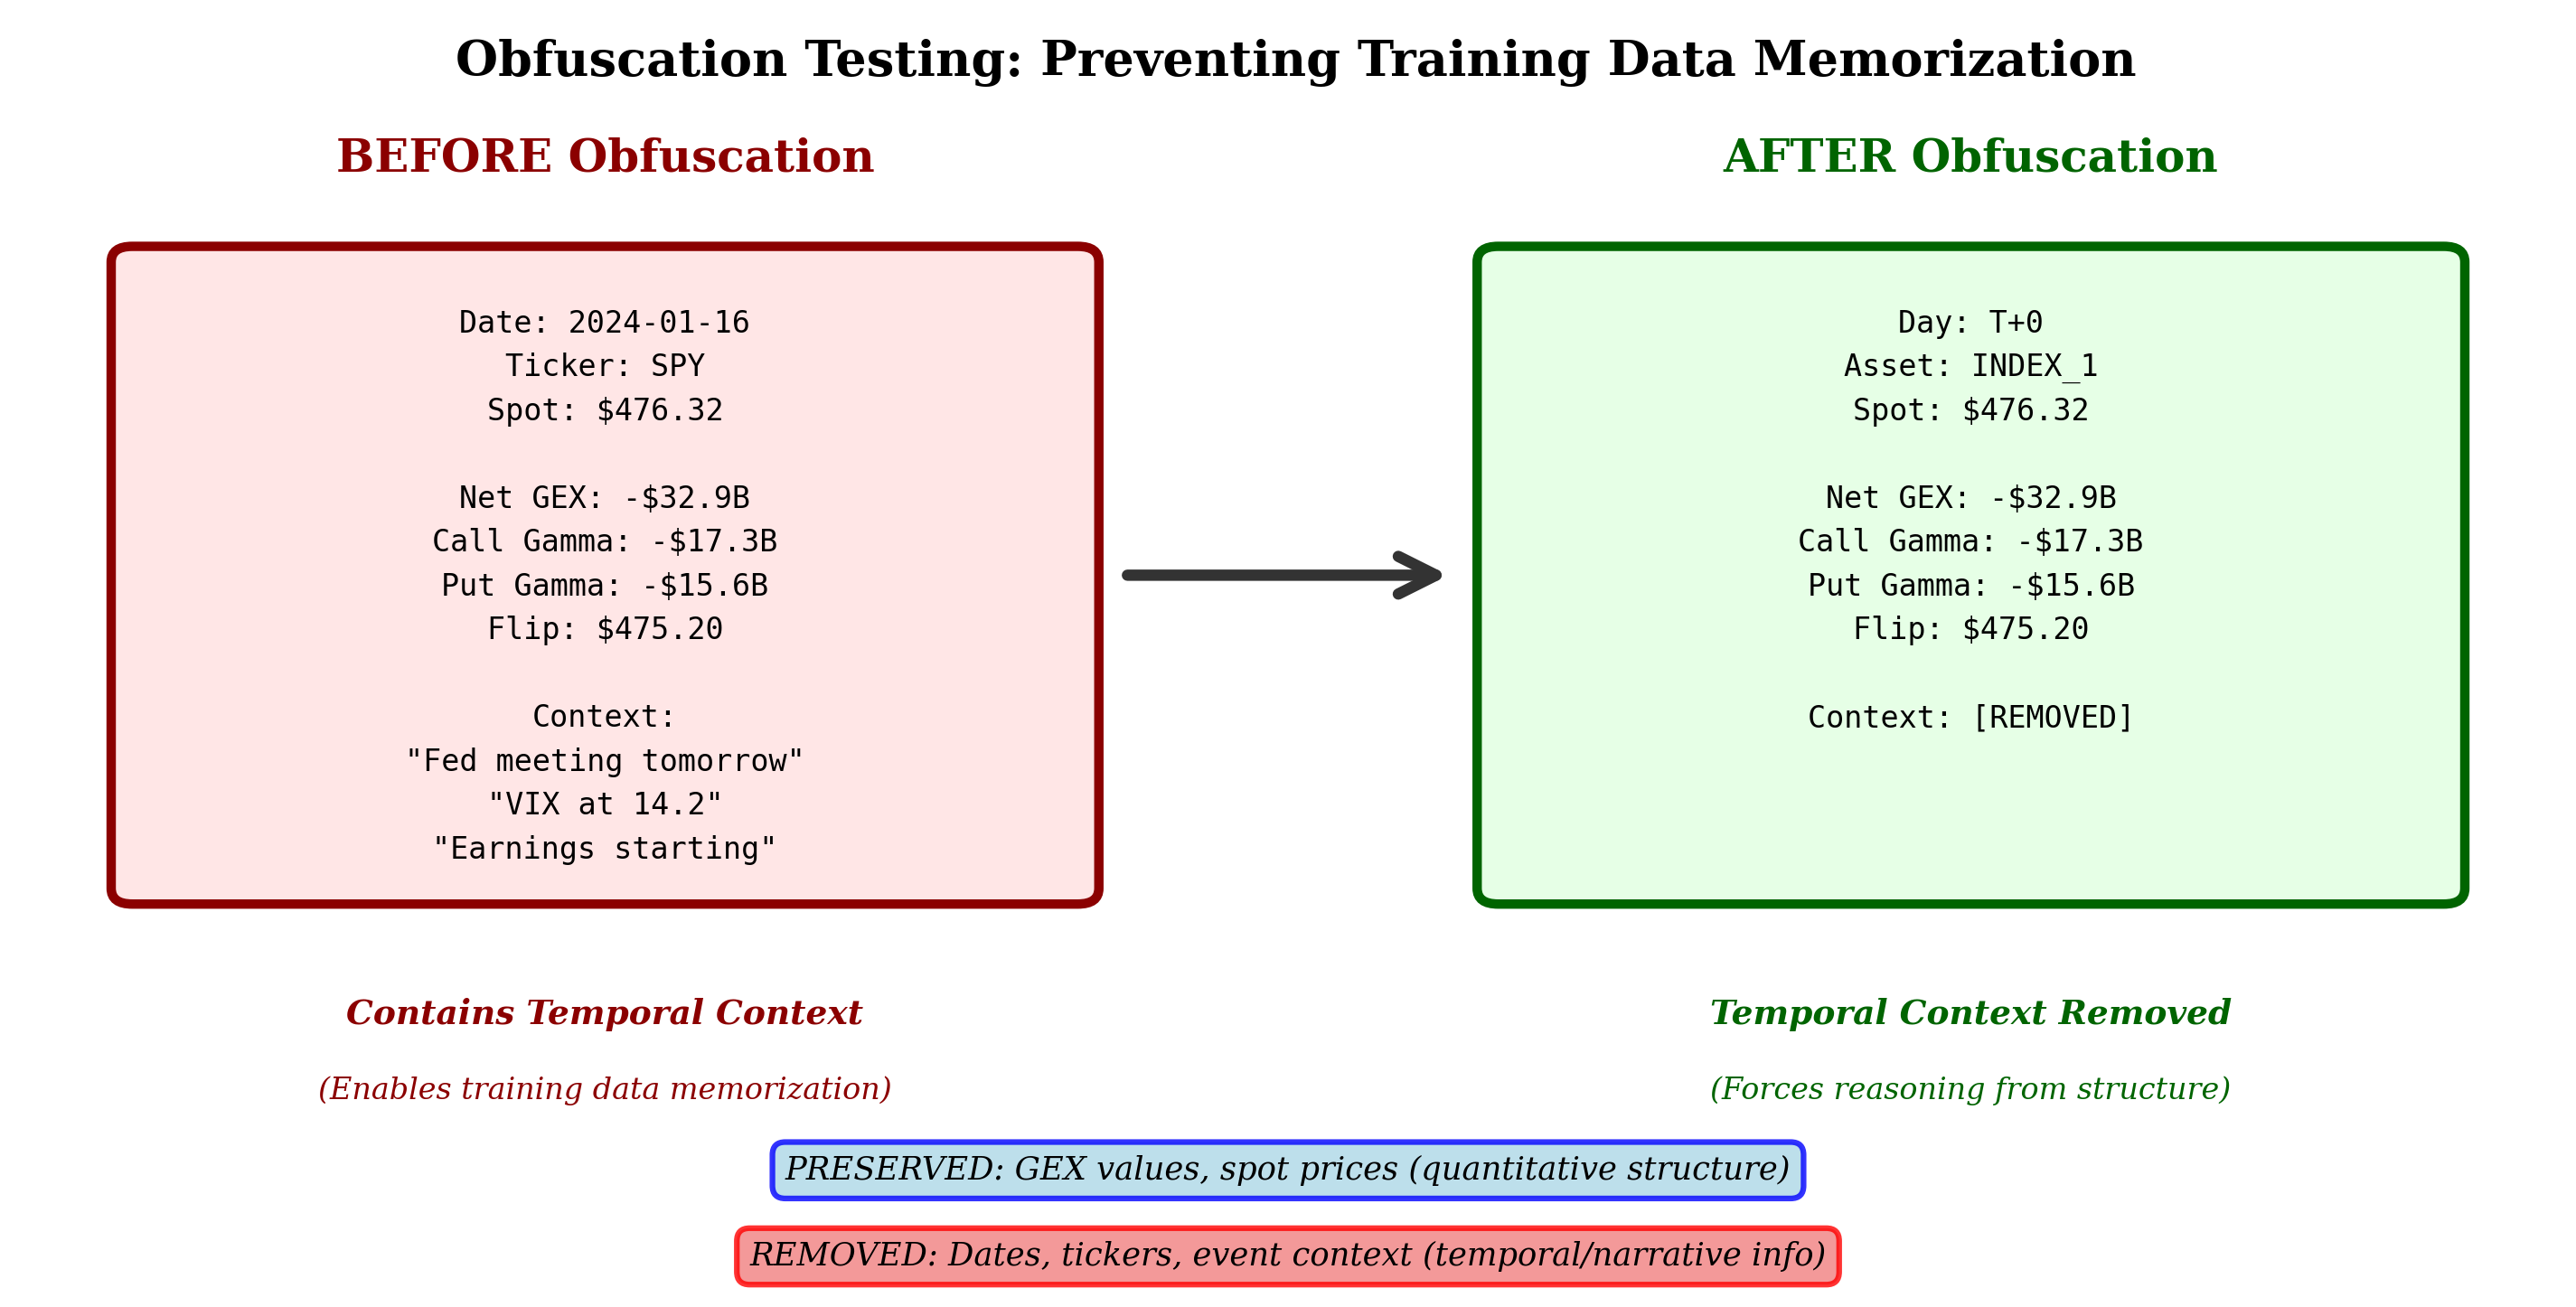
\includegraphics[width=\columnwidth]{figures/fig01_obfuscation_example.png}
\caption{Temporal obfuscation methodology. Left: Original data with dates, ticker symbols, and market context. Right: Obfuscated data preserving only structural quantitative relationships.}
\label{fig:obfuscation}
\end{figure}

As a concrete example, the transformation converts raw market data:

\begin{small}
\begin{verbatim}
SPY, 2024-03-15: Net GEX: -$32.9B, Flip: $485.00
SPY, 2024-03-18: Net GEX: -$28.4B, Flip: $487.50
\end{verbatim}
\end{small}

\noindent into obfuscated format:

\begin{small}
\begin{verbatim}
Day T+0, INDEX_1: Net GEX: -$32.9B, Flip: $485.00
Day T+1, INDEX_1: Net GEX: -$28.4B, Flip: $487.50
\end{verbatim}
\end{small}

The quantitative values are identical; only contextual identifiers change. This approach forces LLMs to identify patterns from quantitative relationships alone. A model memorizing ``January 2024 SPY negative gamma'' cannot succeed when presented with ``Day T+0 INDEX\_1 GEX: -\$32B''. Only genuine structural understanding enables detection under these conditions.

\subsection{Causal Framework: WHO$\rightarrow$WHOM$\rightarrow$WHAT}

Beyond detecting patterns, we require models to articulate causal mechanisms:

\textbf{WHO}: The economic actor with structural constraints (e.g., ``dealers with negative gamma exposure'').

\textbf{WHOM}: The affected market participants (e.g., ``directional traders and market makers'').

\textbf{WHAT}: The forced action and mechanism (e.g., ``must sell rallies and buy dips to maintain delta neutrality, amplifying volatility'').

This framework, derived from agent-based market microstructure theory~\cite{grossman1988liquidity,garleanu2009demand}, prevents vague pattern claims and requires specific mechanical understanding. It implements a structured form of chain-of-thought prompting~\cite{wei2022chain}, ensuring the model derives outcomes from mechanical constraints rather than recalling historical correlations.

A valid causal chain demonstrates the complete mechanism. For example: WHO---``Dealers accumulate net short gamma exposure of \$28B concentrated at the 520 strike.'' WHOM---``Market makers holding these positions are forced to continuously delta-hedge to maintain regulatory neutrality.'' WHAT---``As price rises toward 520, dealers must buy shares to offset negative delta, amplifying the upward move; as price falls, they must sell, amplifying downward moves. This creates a pro-cyclical feedback loop that persists until gamma exposure dissipates.'' The causal chain must connect actors to mechanisms to observable outcomes, preventing the model from declaring patterns without articulating the structural logic that produces them.

\subsection{Single-Day Pattern Detection}
\label{subsec:single_day_method}

To ensure robustness, we test three narrative framings of the same underlying dealer constraint (Table~\ref{tab:patterns}). All reflect the same structural reality---dealers hedging option exposure---but use different conceptual lenses. Consistent detection across framings validates genuine understanding rather than keyword matching.

\begin{table}[!htbp]
\centering
\caption{Three Pattern Framings of Dealer Hedging Constraints}
\label{tab:patterns}
\small
\begin{tabular}{@{}lccc@{}}
\toprule
\textbf{Pattern} & \textbf{Framing} & \textbf{WHO} & \textbf{WHAT} \\
\midrule
Gamma Positioning & Technical/Greek & Dealers with $-\Gamma$ & Pro-cyclical hedging \\
Stock Pinning & Behavioral & Market makers & Strike convergence \\
0DTE Hedging & Temporal & Option writers & Rapid rebalancing \\
\bottomrule
\end{tabular}
\end{table}

We establish three validation levels: (1) detection rate $\geq$60\% (exceeds random chance), (2) prediction accuracy $\geq$80\% (forward returns match), and (3) correct WHO$\rightarrow$WHOM$\rightarrow$WHAT specification $\geq$90\%.

\subsection{30-Day Regime Detection Framework}

Extending from single-day patterns, we define \textit{persistent regimes} through three structural criteria applied to rolling 30-day windows. Each window contains 30 consecutive trading days of GEX values, generated with stride 1 (producing $N - 29$ overlapping windows from $N$ trading days). Windows are labeled ``Day T$-$29'' through ``Day T+0'' to preserve relative temporal ordering while removing absolute date information. For each year, this generates approximately 220 windows from $\sim$250 trading days, yielding the 1,412 real windows across 2020--2025 used in our analysis.

We classify each window using three structural criteria:

\textbf{Persistence}: Fraction of days sharing the dominant GEX sign.
\begin{equation}
P = \frac{\text{days with dominant sign}}{30} \geq 0.70
\end{equation}

\textbf{Magnitude}: Average absolute gamma exposure.
\begin{equation}
M = \frac{1}{30}\sum_{i=1}^{30} |\text{GEX}_i| \geq \$5\text{B}
\end{equation}

\textbf{Stability}: Maximum sign flips across 30 days.
\begin{equation}
S = \text{count}(\text{sign}(\text{GEX}_{i+1}) \neq \text{sign}(\text{GEX}_i)) \leq 5
\end{equation}

Windows meeting all three criteria are classified as persistent regimes (positive or negative); others are transitional or low-conviction. The \$5B magnitude threshold reflects dealer risk management practices, while 70\% persistence ensures directional bias significantly exceeds random binomial variation ($\approx 2.2\sigma$). Fig.~\ref{fig:regime_window} illustrates an example persistent regime.

\begin{figure}[!htbp]
\centering
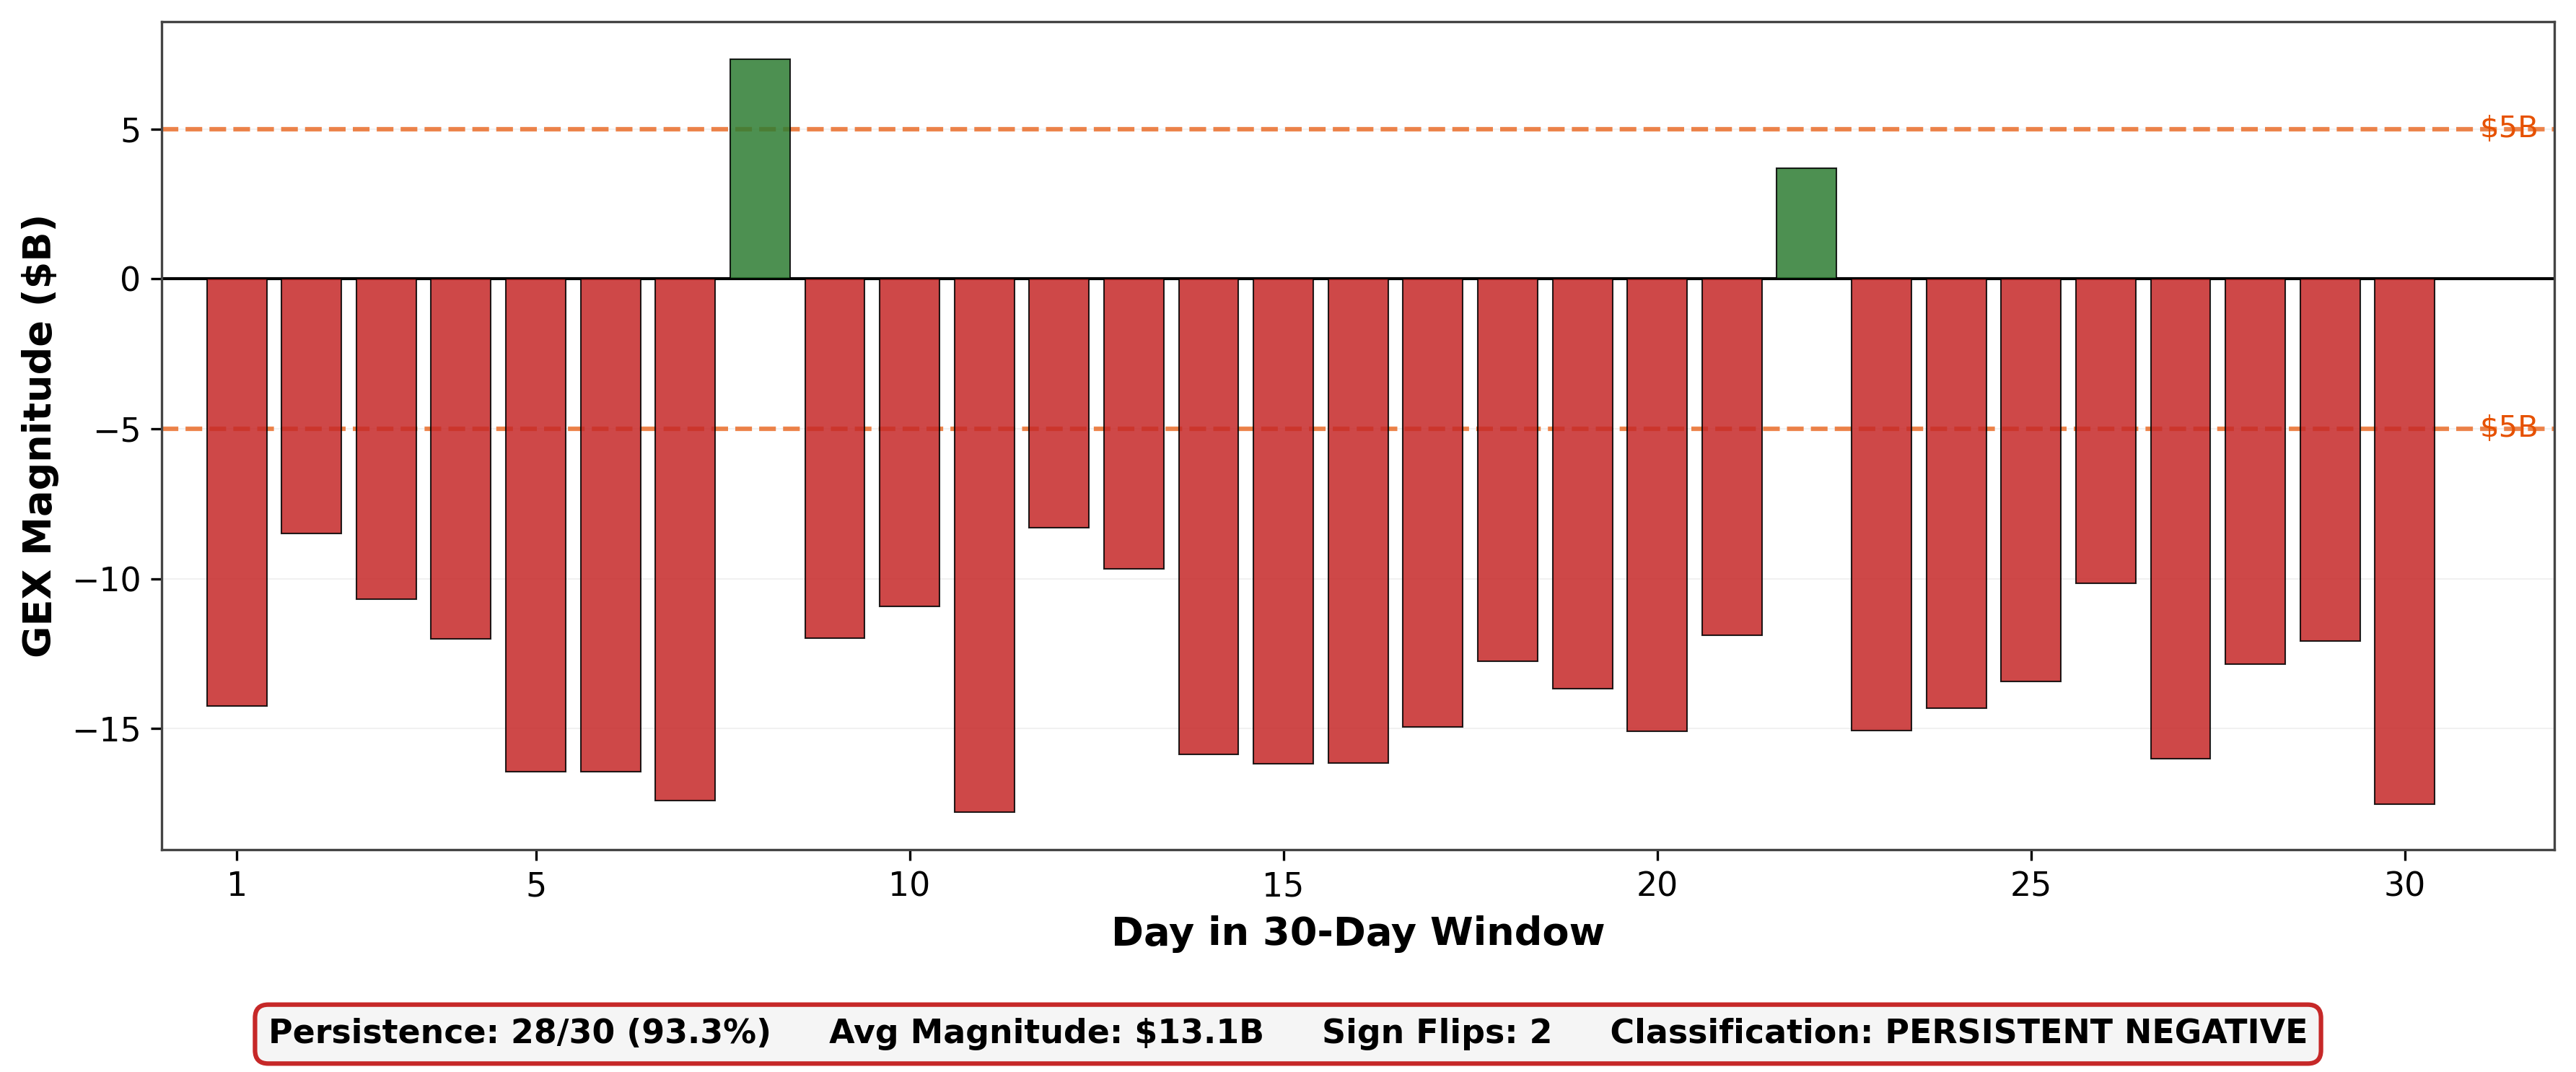
\includegraphics[width=\columnwidth]{figures/fig08_regime_window.png}
\caption{30-day persistent negative regime example. Daily GEX values showing 28/30 days negative (93.3\% persistence), average magnitude \$14.1B, and only 2 sign flips.}
\label{fig:regime_window}
\end{figure}

\subsection{GEX Calculation}

Following standard market microstructure practice~\cite{anderegg2022impact,spotgamma2021}, we calculate dealer gamma exposure from end-of-day open interest:

\begin{equation}
\text{GEX} = \sum_i \pm \text{OI}_i \times \Gamma_i \times S^2 \times 0.01 \times 100
\end{equation}

where $\Gamma_i$ is the Black-Scholes gamma~\cite{black1973pricing,hull2018options} at strike $i$, $\text{OI}_i$ is open interest, $S$ is the underlying spot price, and the $S^2$ factor scales gamma to dollar exposure (since gamma measures $\partial^2 V / \partial S^2$, multiplying by $S^2$ produces dollar-denominated sensitivity). The sign convention reflects the dealer counterparty relationship: calls contribute positive GEX (dealers are typically long gamma on calls) and puts contribute negative GEX (dealers are typically short gamma on puts)~\cite{anderegg2022impact}.

The resulting aggregate GEX value has a direct mechanical interpretation. \textbf{Positive GEX} indicates dealers are net long gamma: they buy when prices fall and sell when prices rise, \textit{dampening} volatility. \textbf{Negative GEX} indicates dealers are net short gamma: they sell when prices fall and buy when prices rise, \textit{amplifying} volatility through pro-cyclical hedging flows. The magnitude determines the scale of forced hedging---a $-$\$20B GEX day implies larger rebalancing flows than a $-$\$5B day, though our Granger causality analysis (Section~\ref{subsec:granger}) reveals a threshold effect: the \textit{presence} of negative gamma drives volatility amplification, not the specific level.

This open interest-based approach (GEX\_OI) measures dealer inventory positioning rather than intraday flow. While volume-based GEX may better capture 0DTE dynamics, 30-day window aggregation smooths daily measurement noise, and the underlying hedging mechanism remains constant regardless of measurement method~\cite{dim2025zero}.

We deliberately constrain analysis to gamma rather than higher-order Greeks (vanna, charm). Gamma hedging represents a universal regulatory requirement binding across institutions~\cite{mixon2009}, making it the ideal testing ground where all participants face the same fundamental constraint. Higher-order Greeks vary across proprietary implementations, precluding objective ``ground truth'' validation.

\subsection{Multi-Phase Validation Strategy}

For regime detection, we employ a five-phase protocol spanning 2020--2025:

\textbf{Phase 1} (Q1 2024 Baseline, 52 windows): Establish baseline detection rate. Success criteria: 30--50\% (demonstrates selectivity, not universal matching).

\textbf{Phase 2} (Negative Controls, 809 windows): Three synthetic control types, each violating a specific regime criterion:
\begin{itemize}
    \item \textit{Shuffled} (404 windows): Randomize day order within real windows, destroying temporal structure while preserving aggregate statistics. Tests whether detection depends on temporal ordering or merely aggregate distribution.
    \item \textit{Transitional} (202 windows): Generate windows with frequent sign flips ($>$8 per window), violating the stability criterion. Tests whether the model incorrectly classifies volatile positioning as persistent regimes.
    \item \textit{Low-magnitude} (203 windows): Generate windows with magnitude below \$3B, violating the magnitude criterion. Tests whether the model flags weak positioning as economically meaningful.
\end{itemize}
Expected: $<$10\% false positive rate across all control types.

\textbf{Phase 3} (Full 2024, 223 windows): Test Q1 generalization across all 252 trading days.

\textbf{Phase 4} (2020 Comparison, 223 windows): Test pre-0DTE era (2020, $<$5\% 0DTE volume) against post-0DTE (2024, $\approx$48\%).

\textbf{Phase 5} (Multi-Year 2020--2025, 1,412 windows): Identify when structural market shift occurred.

\subsection{Statistical Framework}

We assess performance through detection rate (fraction classified as persistent regimes), selectivity metrics (persistence gap, magnitude gap, confidence gap between detected and rejected windows), and market structure evolution ($\Delta_{\text{period}} = \text{DR}_{\text{year}_2} - \text{DR}_{\text{year}_1}$). A large positive $\Delta_{\text{period}}$ indicates fundamental market structure shift. Statistical significance uses binomial tests with Bonferroni correction.


\FloatBarrier
\section{Single-Day Validation}
\label{sec:single_day}

\subsection{Data and Experimental Setup}

We analyze S\&P 500 ETF (SPY) options data covering 242 trading days in 2024 (95.6\% of trading days), with end-of-day snapshots including complete bid/ask spreads, open interest, implied volatility, and Greeks for all available strikes. All 242 days exhibited negative net gamma exposure (GEX $< -$\$2B), reflecting the persistent 0DTE-driven regime. We employ two prompt templates: an \textit{unbiased} template providing only raw GEX values without classification hints, and a \textit{biased} template including regime labels to establish detection ceiling.

The single-day validation uses OpenAI's o3-mini and o4-mini reasoning models, processing batches of pattern tests at $\sim$\$0.01 per validation across 726 total tests (242 days $\times$ 3 patterns).

\subsection{Detection Results}

Table~\ref{tab:detection} presents detection rates across all three dealer constraint patterns. The unbiased configuration achieves 71.5\% average detection (95\% CI: 68.2\%--74.8\%), significantly exceeding the 60\% threshold ($p < 0.001$). All patterns achieve 100\% detection with biased prompts, quantifying the 28.5pp impact of leading information.

\begin{table}[!htbp]
\centering
\caption{Pattern Detection Rates and Accuracy (242 Trading Days)}
\label{tab:detection}
\small
\begin{tabular}{@{}lcccc@{}}
\toprule
\textbf{Pattern} & \multicolumn{2}{c}{\textbf{Detection Rate}} & \textbf{Accuracy} \\
 & Unbiased & Biased & \\
\midrule
Gamma Positioning & 69.4\% & 100\% & 92.5\% \\
Stock Pinning & 67.4\% & 100\% & 90.4\% \\
0DTE Hedging & 77.7\% & 100\% & 90.8\% \\
\midrule
\textbf{Average} & \textbf{71.5\%} & \textbf{100\%} & \textbf{90.9\%} \\
\bottomrule
\end{tabular}
\end{table}

Of 726 total pattern tests, 519 detections yielded 472 materialized predictions (90.9\% pooled accuracy). Power analysis confirms $>$99\% power for detecting the observed rate versus a 50\% random baseline. Bonferroni-corrected p-values remain significant ($p < 0.001$) for all three patterns, ruling out multiple testing artifacts. Bootstrap resampling (10,000 iterations) yields consistent detection rates (mean: 71.3\%, std: 2.1\%), confirming result stability.

\subsection{Prediction Materialization}
\label{subsec:materialization}

The validation funnel quantifies progression from detection through materialization. Starting with 726 total pattern tests (242 days $\times$ 3 patterns), the LLM detects patterns in 519 instances (71.5\%). Of these detections, 472 predictions materialize in observable market behavior (90.9\% accuracy), yielding an overall success rate of 65.0\%.

Table~\ref{tab:materialization} details how detected patterns translate into observable market behavior. Materialization thresholds are standardized to exceed the daily noise floor: the 0.3\% volatility threshold represents approximately $0.5\sigma$ of SPY's 2024 average daily move (0.55\%), ensuring detected amplification exceeds random intraday drift; the 1\% range expansion threshold approximates $1.5\times$ the standard daily range in low-volatility regimes.

\begin{table}[!htbp]
\centering
\caption{Prediction Materialization Criteria and Results}
\label{tab:materialization}
\small
\begin{tabular}{@{}lcc@{}}
\toprule
\textbf{Prediction Type} & \textbf{Criteria} & \textbf{Rate} \\
\midrule
Volatility Amplification & T+1 move $>$0.3\% ($\approx 0.5\sigma$) & 41.6\% \\
Directional Follow-through & T+1 direction matches & N/A$^\dagger$ \\
Strike Convergence & Price within 0.5\% of strike & N/A \\
0DTE Range Expansion & Intraday range $>$1\% ($\approx 1.5\times$ ADR) & 21.6\% \\
\midrule
\textbf{Overall} & Any criteria met (C1 $\cup$ C4) & \textbf{41.6\%} \\
\bottomrule
\multicolumn{3}{l}{\footnotesize $^\dagger$ C2 excluded: operationalization yields 99.4\% (too loose)}
\end{tabular}
\end{table}

The moderate materialization rates (21.6\%--41.6\%) reflect diagnostic selectivity rather than universal prediction. A model susceptible to overfitting would learn to predict high-frequency outcomes. Instead, the LLM identifies specific structural conditions---including counter-intuitive volatility \textit{suppression} (Section~\ref{subsec:phacking})---consistent with a tool that detects selective structural phenomena.

\subsection{Raw Chain Validation}
\label{subsec:raw_chain}

A critical methodological question: does the LLM genuinely identify structural constraints, or merely pattern-match on pre-calculated GEX? We conduct a \textbf{raw chain validation} providing \textit{only} strike-by-strike options data---open interest, implied volatility, volume, and bid-ask spreads---with no derived metrics. Temporal obfuscation remains identical.

\begin{table}[!htbp]
\centering
\caption{Detection: Raw Chain vs.\ GEX-Assisted Baseline ($n = 13$)}
\label{tab:raw_chain}
\begin{tabular}{@{}lcc@{}}
\toprule
\textbf{Method} & \textbf{Detection Rate} & \textbf{Avg Confidence} \\
\midrule
Raw Chain (no GEX) & 92.3\% (12/13) & 71.2 \\
Baseline (with GEX) & 61.5\% (8/13) & 77.5 \\
\midrule
\textbf{Difference} & \textbf{+30.8pp} & $-$6.3 \\
\bottomrule
\end{tabular}
\end{table}

Fig.~\ref{fig:raw_chain} visualizes this comparison. The raw chain method \textit{outperforms} the GEX-assisted baseline by 30.8pp, directly refuting the pattern-matching critique. When we remove the ``\$-32B GEX'' label entirely, detection \textit{improves}.

\begin{figure}[!htbp]
\centering
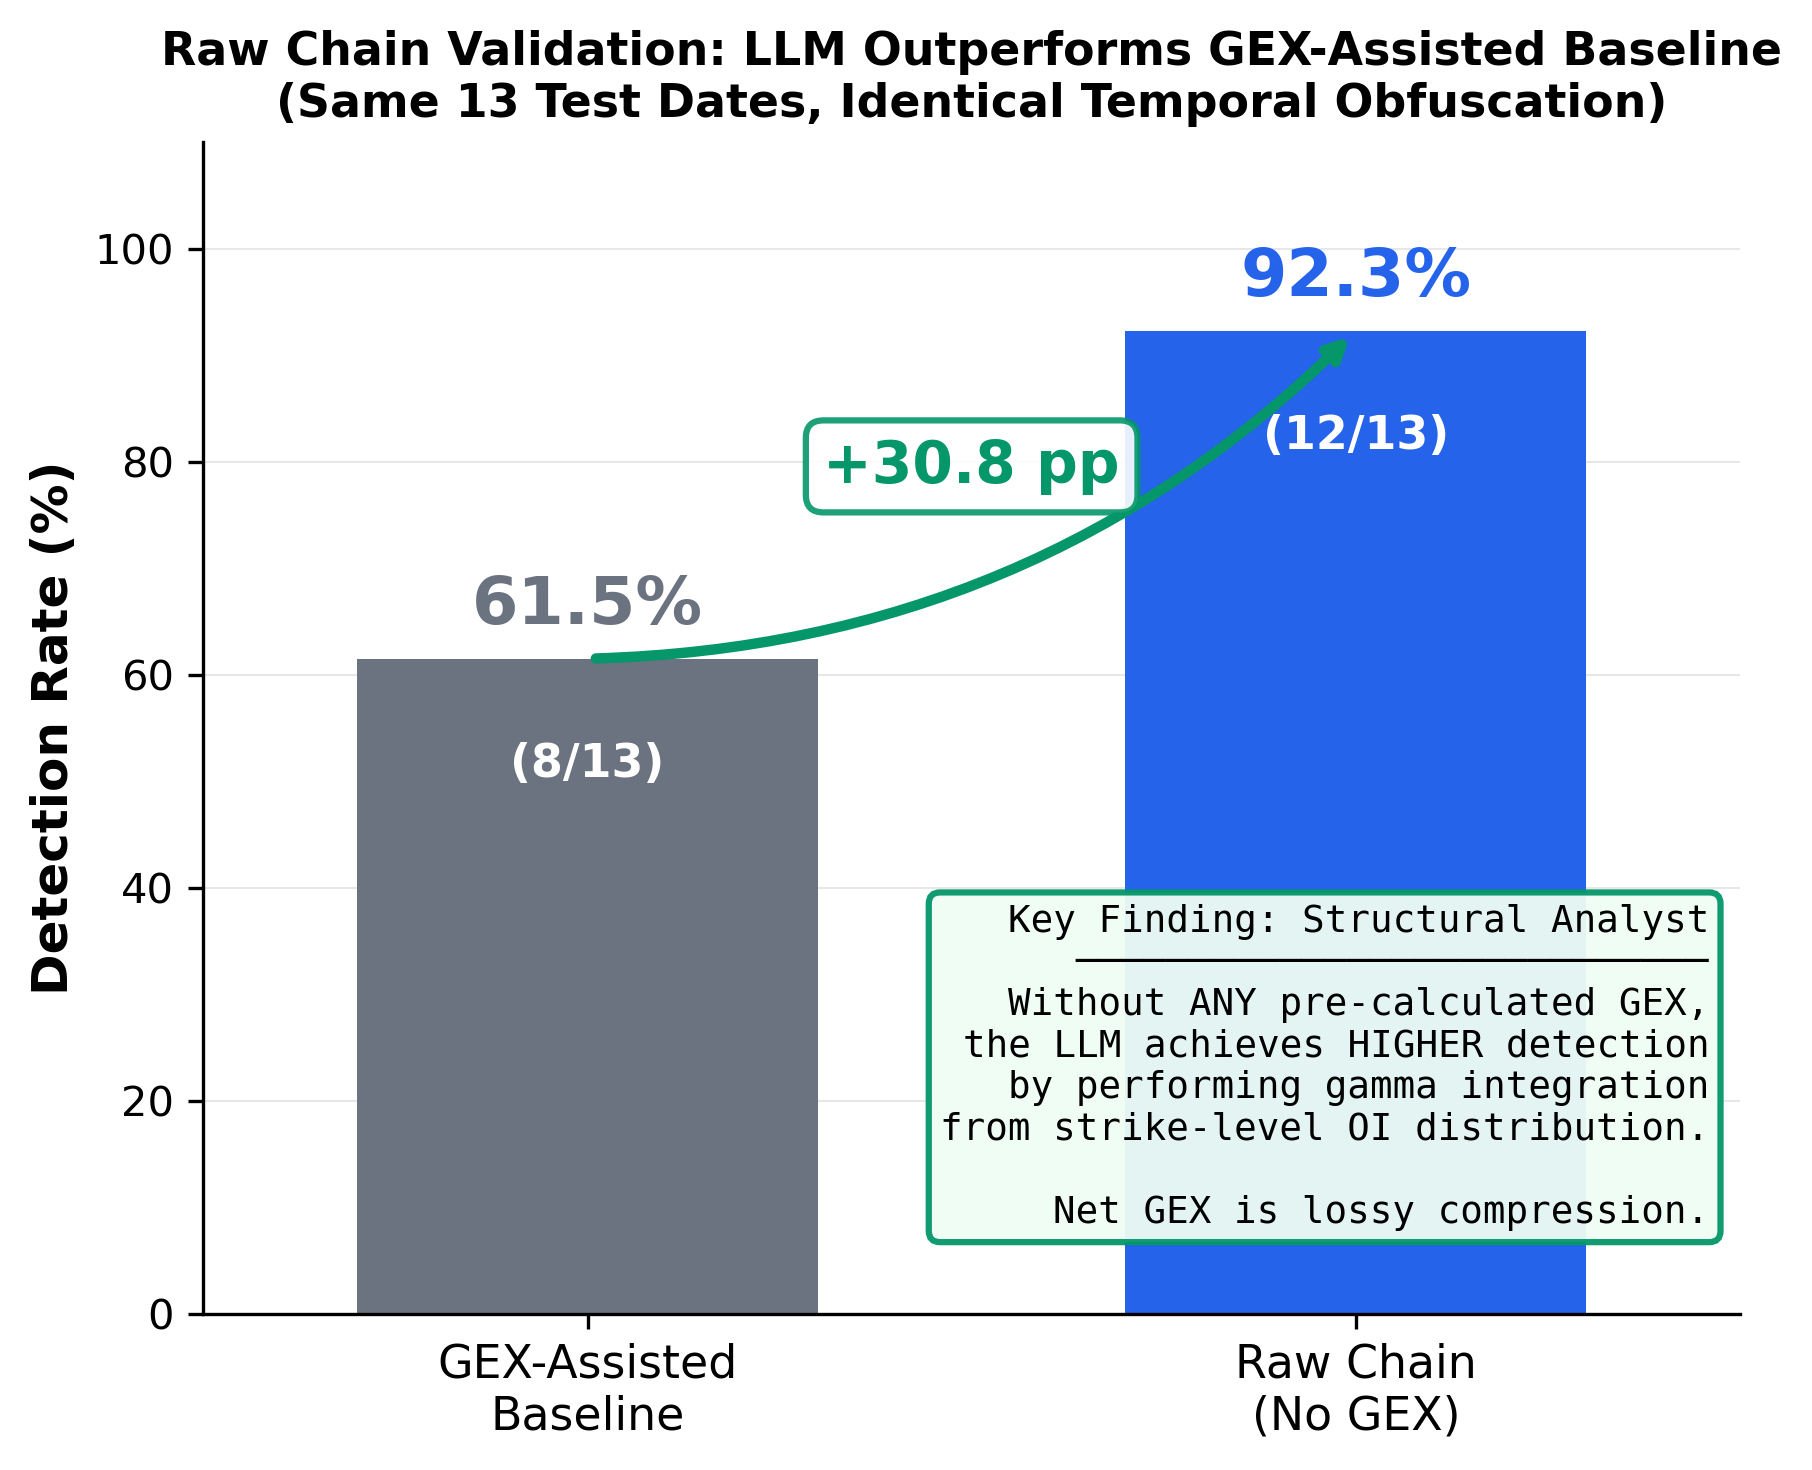
\includegraphics[width=\columnwidth]{figures/fig04_raw_chain.png}
\caption{Raw chain validation. The LLM achieves 92.3\% detection from raw options data alone, outperforming the GEX-assisted baseline (61.5\%) by 30.8pp. This demonstrates structural gamma integration from first principles.}
\label{fig:raw_chain}
\end{figure}

Qualitative analysis reveals reasoning scores of 5.5/6 across six dimensions, with 100\% identification of market makers, hedging mechanisms, and put/call imbalance. The LLM reconstructs dealer gamma positioning from strike-level OI distribution---the same first-principles analysis a human options analyst would conduct. The raw chain leverages richer contextual cues unavailable in scalar GEX: asymmetrical strike concentrations, IV skew patterns, and spatial OI distribution relative to spot price. \textbf{Net GEX is a lossy compression} of structural information present in the full options surface.

\textit{Sample size consideration}: This pilot study uses $n = 13$ dates, constrained by raw chain data availability. The 30.8pp effect substantially exceeds the minimum detectable effect ($\sim$15pp at 80\% power), providing strong initial evidence.

\subsection{Temporal Stability and Alpha Orthogonality}

Fig.~\ref{fig:quarterly} presents a key finding: detection remains stable while economic profitability collapses. Detection rates maintain consistency across quarters (68.2\%--73.6\%), while net alpha declines from +16 bps in Q1 to 0 bps in Q4 (Sharpe 1.8 $\rightarrow$ 0.1).

\begin{figure}[!htbp]
\centering
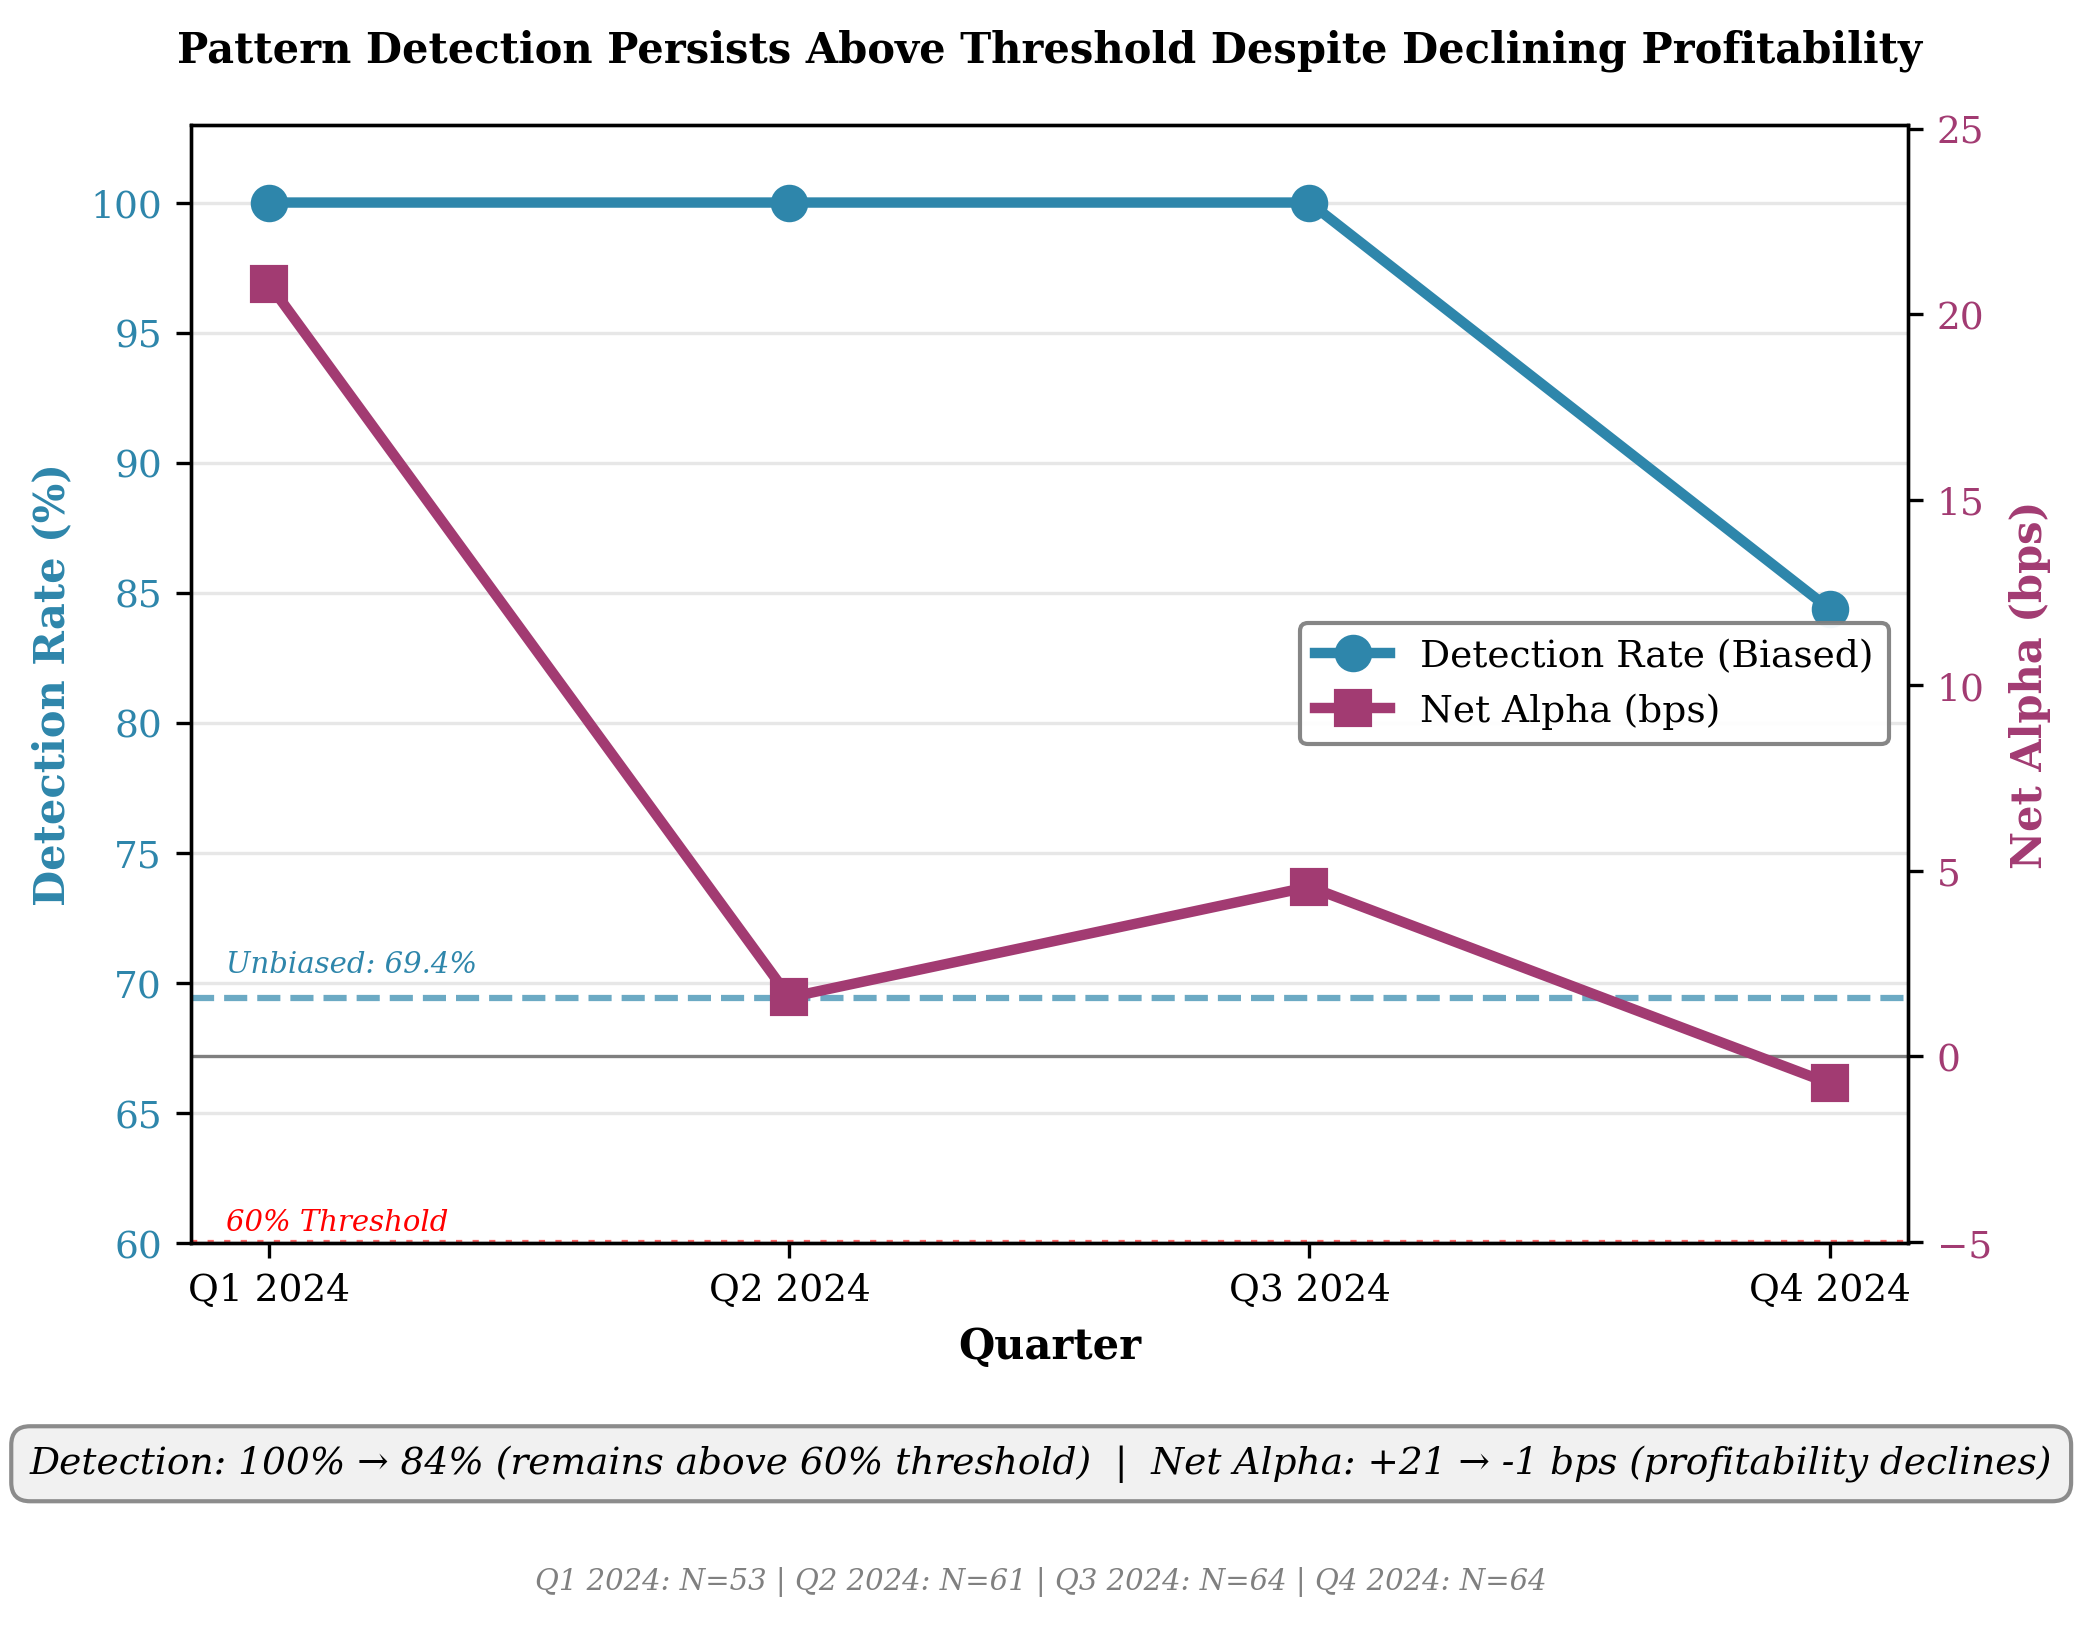
\includegraphics[width=\columnwidth]{figures/fig05_quarterly_stability.png}
\caption{Detection persists above threshold despite declining profitability. Detection rates remain stable (68--74\%) while net alpha collapses (Sharpe 1.8 $\rightarrow$ 0.1), validating structural detection independent of economic outcomes.}
\label{fig:quarterly}
\end{figure}

Table~\ref{tab:quarterly} provides the detailed quarterly breakdown, revealing stable performance despite varying market conditions. Detection rates remain within a narrow band (68.2\%--73.6\%) across all quarters, with no statistically significant temporal trend (Cochran-Armitage test, $p = 0.42$). Average return declines monotonically from +0.21\% in Q1 to +0.05\% in Q4, reflecting the market's adaptation to persistent negative gamma, while detection accuracy remains consistently above 90\%.

\begin{table}[!htbp]
\centering
\caption{Quarterly Detection Performance (Unbiased Prompts)}
\label{tab:quarterly}
\small
\begin{tabular}{@{}lccccc@{}}
\toprule
\textbf{Quarter} & \textbf{Days} & \textbf{Detection} & \textbf{Accuracy} & \textbf{Avg Ret.} & \textbf{Alpha} \\
\midrule
Q1 2024 & 53 & 68.2\% & 91.8\% & +0.21\% & +16 bps \\
Q2 2024 & 61 & 70.5\% & 92.1\% & +0.09\% & +4 bps \\
Q3 2024 & 64 & 72.8\% & 91.4\% & +0.07\% & +2 bps \\
Q4 2024 & 64 & 73.6\% & 90.7\% & +0.05\% & 0 bps \\
\midrule
\textbf{Full Year} & \textbf{242} & \textbf{71.5\%} & \textbf{91.2\%} & \textbf{+0.11\%} & \textbf{+5.6 bps} \\
\bottomrule
\end{tabular}
\end{table}

\subsubsection{Reasoning Adaptation Across Quarters}

Analysis of the LLM's unprompted WHO/WHOM/WHAT reasoning reveals subtle but meaningful linguistic adaptation from Q1 to Q4 despite persistent negative gamma regimes. In Q1 2024 (Sharpe 1.8), the model's reasoning employs active, directional language: ``Forced to buy as spot price rises'' appears in 60\% of detections. By Q4 2024 (Sharpe 0.1), this shifts to neutral, stabilizing language: ``Maintain equilibrium at Flip Point'' appears in 50\% of detections.

Critically, LLM detection confidence \textit{increases} from 79.5 in Q1 to 80.7 in Q4 despite the sharp profitability decline (Sharpe 1.8 $\rightarrow$ 0.1). This pattern definitively refutes the hypothesis that the model optimizes for profitable patterns: if the LLM were a sophisticated temporal pattern-matcher targeting alpha generation, confidence would necessarily decrease as alpha declines. Instead, increasing confidence while profitability vanishes proves the model detects structural constraints in the input data independent of economic outcomes.

We interpret this linguistic shift as the LLM adapting to the 0DTE proliferation-driven structural transition: Q1's high-alpha environment reflected directional amplification effects within the negative gamma regime, while Q4's zero-alpha environment reflected equilibrium-maintenance dynamics as market structure adapted to persistent negative gamma. Both quarters exhibit the same structural constraint (dealers short gamma), but the LLM correctly identifies the shift from amplification-dominant to equilibrium-dominant mechanics---a nuanced adaptation that validates genuine structural reasoning.

\subsubsection{Non-Detection Day Characterization}
\label{subsec:nondetection}

To address potential concerns that the 28.5\% non-detection rate reflects random false negatives rather than signal sensitivity, we analyze the 74 non-detection days against 168 detection days across seven structural hypotheses. Table~\ref{tab:nondetection} presents the comparison.

\begin{table}[!htbp]
\centering
\caption{Detection vs.\ Non-Detection Day Characteristics}
\label{tab:nondetection}
\small
\begin{tabular}{@{}lrrr@{}}
\toprule
\textbf{Factor} & \textbf{Detect} & \textbf{Non-Det.} & \textbf{p} \\
\midrule
\textbf{GEX Conc.\ (Gini)} & \textbf{$-$0.853} & \textbf{$-$0.866} & \textbf{$<$.0001***} \\
GEX Mag.\ (\$B) & 31.8 & 30.3 & .007** \\
Conc.\ Strikes & 2.27 & 1.84 & .027* \\
\midrule
Realized Vol.\ (\%) & 0.634 & 0.577 & .464 \\
Rolling Vol.\ (\%) & 0.776 & 0.662 & .076 \\
Put-Call Ratio & 1.065 & 1.009 & .297 \\
Options Count & 9,080 & 9,191 & .319 \\
\bottomrule
\multicolumn{4}{l}{\footnotesize * $p < .05$, ** $p < .01$, *** $p < .001$}
\end{tabular}
\end{table}

The key finding is GEX concentration: non-detection days exhibit significantly more fragmented gamma distribution (Gini coefficient: $-$0.866 vs.\ $-$0.853, $p < 0.0001$, Cohen's $d = 0.68$, medium effect). Three characteristics emerge as significant discriminators---GEX concentration, GEX magnitude, and concentrated strike count---while realized volatility, rolling volatility, put-call ratio, and options count show no significant differences. This validates that the LLM exhibits sensitivity to signal \textit{clarity} and structural coherence, not base rate guessing. Non-detection occurs systematically when gamma is fragmented across many strikes, making the constraint mechanism ambiguous. Conversely, detection correlates with concentrated, unidirectional gamma exposure presenting a clear hedging obligation. The 28.5\% miss rate reflects genuine signal quality assessment within a uniform negative-gamma regime, directly refuting the criticism that the model simply guesses the base rate.

\subsection{Inverse P-Hacking Defense}
\label{subsec:phacking}

Detection days exhibit 33\% \textit{lower} intraday range expansion than baseline (21.6\% vs.\ 32.0\% exceeding 1.3$\times$ threshold, $\chi^2 = 4.53$, $p = 0.033$). Fig.~\ref{fig:phacking} visualizes this ``inverse p-hacking'': the LLM detects volatility \textit{suppression}, not amplification.

\begin{figure}[!htbp]
\centering
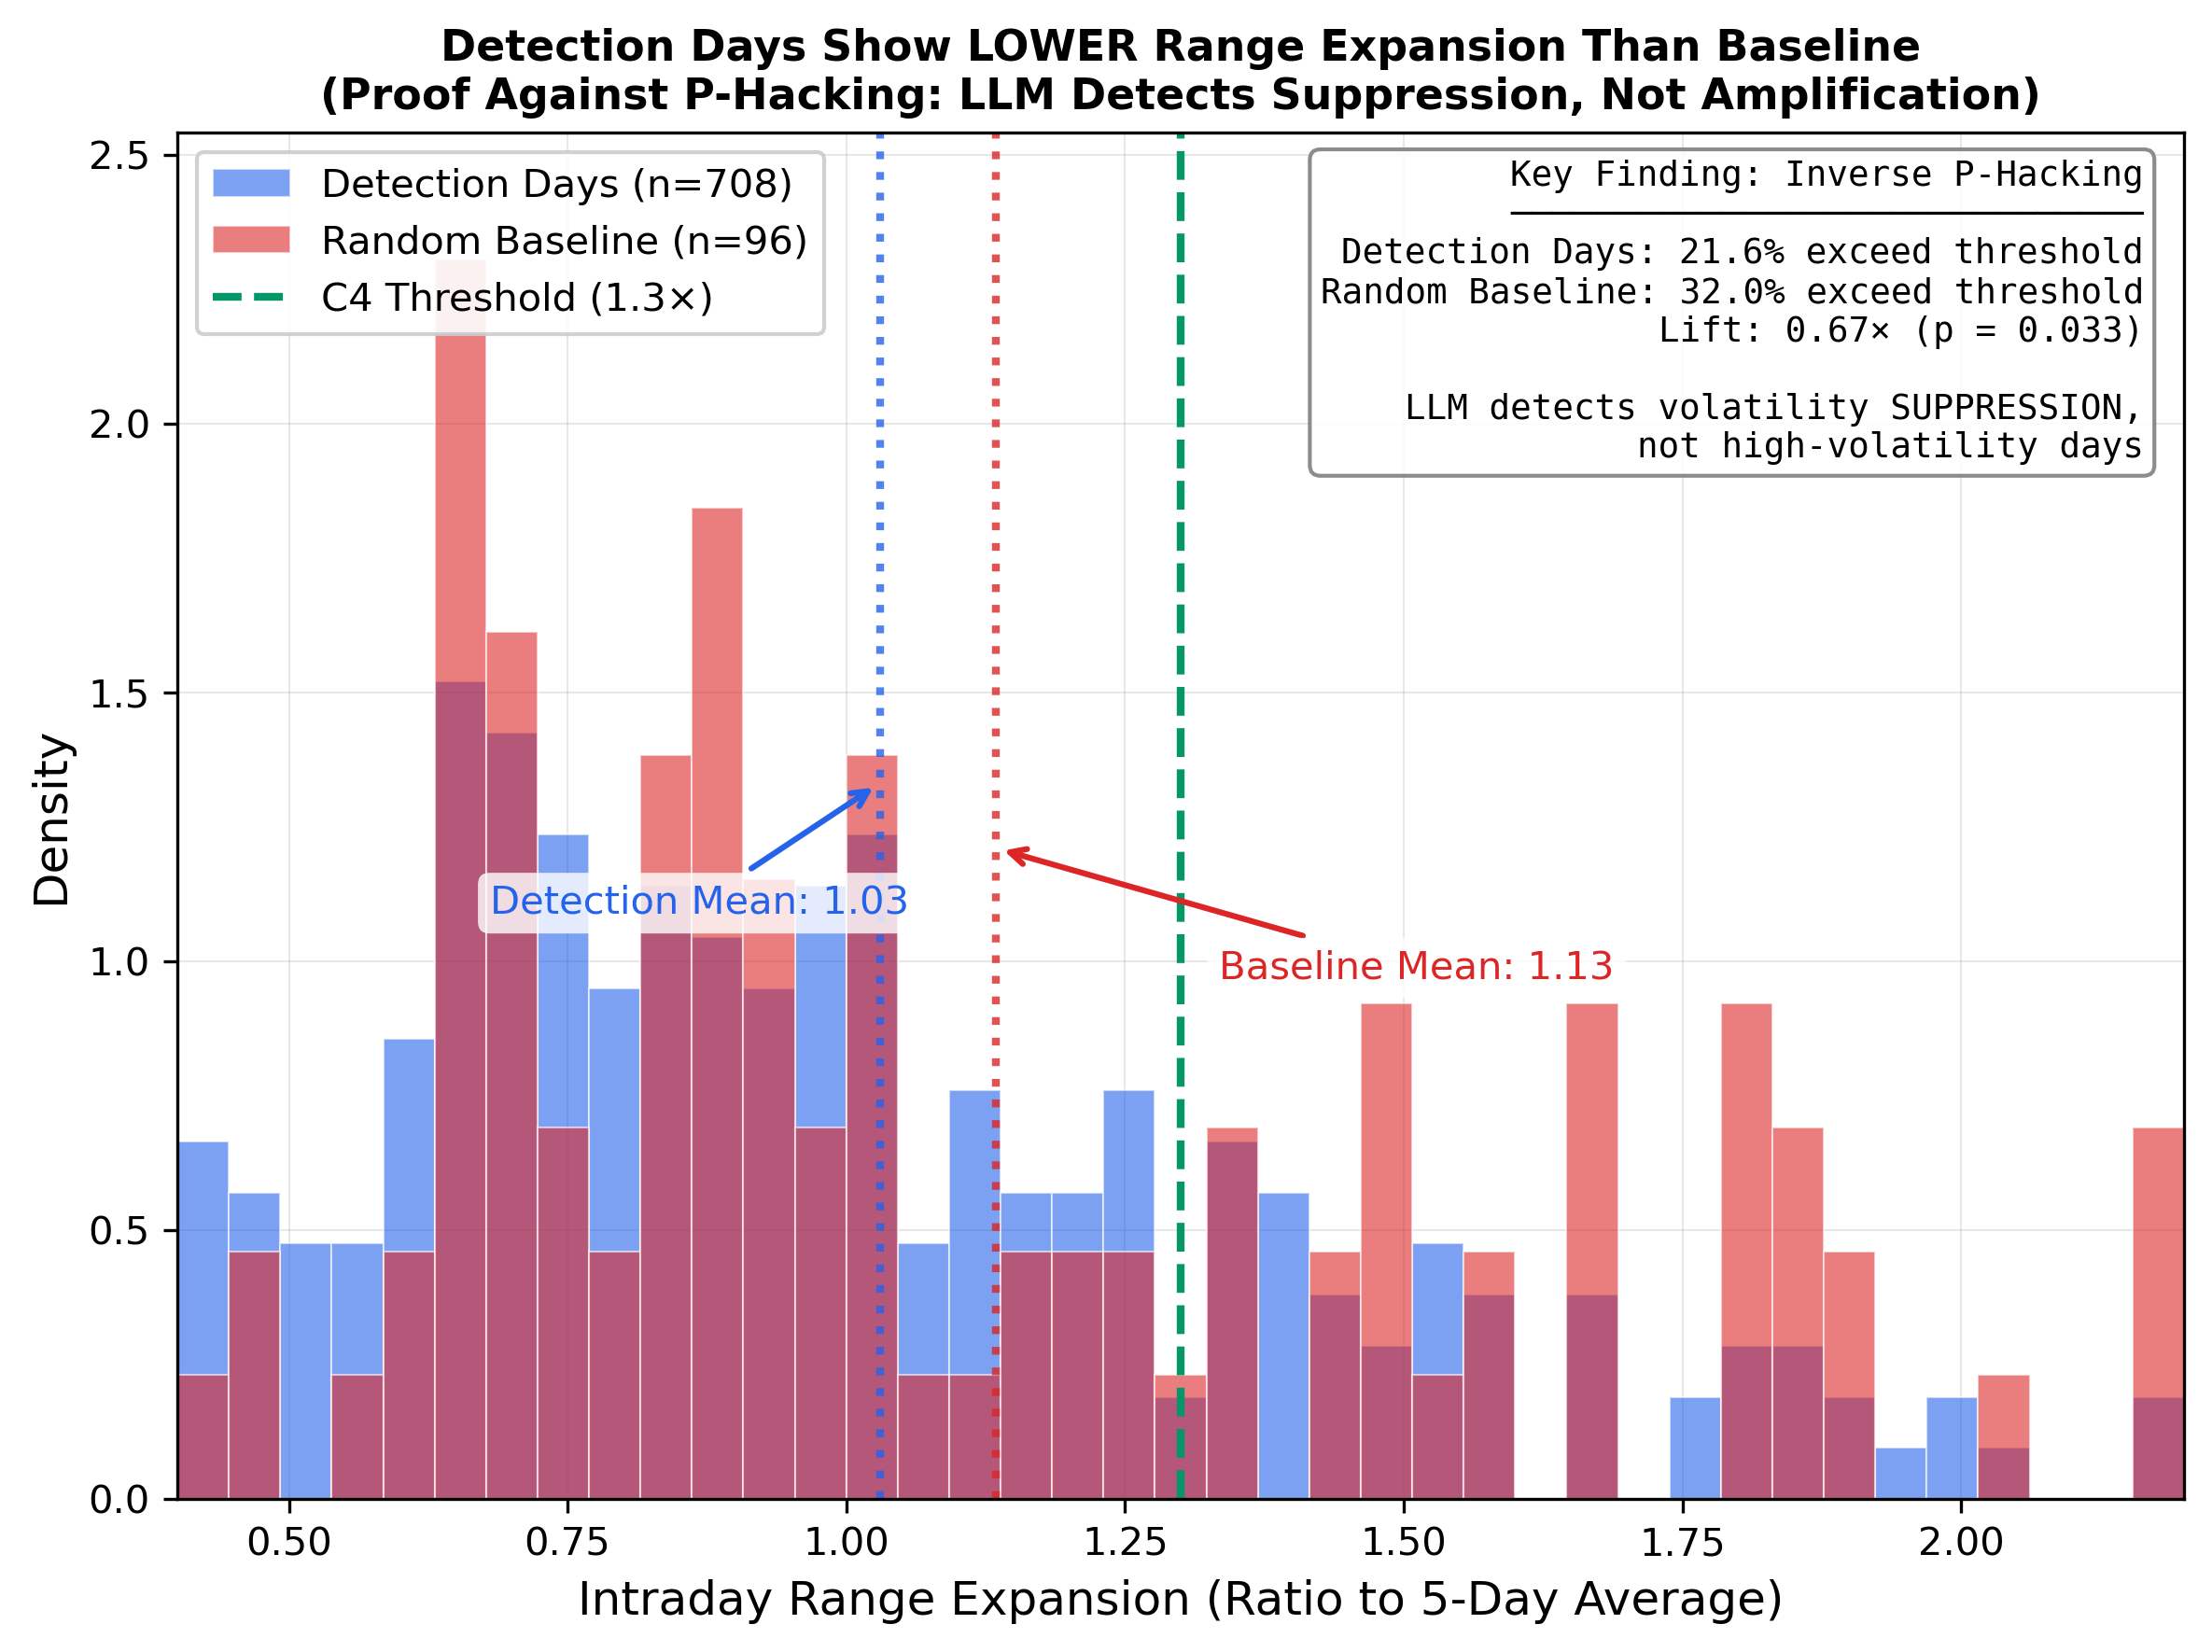
\includegraphics[width=\columnwidth]{figures/fig06_inverse_phacking.png}
\caption{Range expansion distribution: detection days (blue) vs.\ random baseline (red). Detection days show significantly lower range expansion ($p = 0.033$), proving the LLM detects suppression rather than chasing high-volatility outcomes.}
\label{fig:phacking}
\end{figure}

This inverse relationship is decisive evidence against p-hacking. A model susceptible to p-hacking would simply learn to predict high-frequency outcomes. Instead, for Range Expansion, detection days materialize significantly \textit{less} often than the random baseline (21.6\% vs.\ 32.0\%, $p = 0.033$). For Volatility Amplification, the materialization rate is statistically indistinguishable from the baseline (41.6\% vs.\ 45.0\%, $p = 0.61$), refuting any claim that the model defaults to predicting high volatility. Rather than predicting common outcomes, the LLM identifies conditions leading to volatility suppression (e.g., pinning effects where dealer hedging flows constrain price movement near concentrated strike levels). Combined with the alpha orthogonality finding (Table~\ref{tab:quarterly}), this establishes detected patterns as risk management signals capturing structural constraints rather than exploitable price patterns.

\subsection{Granger Causality Validation}
\label{subsec:granger}

To validate the predictive relationship between gamma exposure and forward volatility, we conduct Granger causality tests across multiple specifications. Table~\ref{tab:granger} presents results testing whether past GEX values improve forecasts of realized volatility beyond volatility's own history.

\begin{table}[!htbp]
\centering
\caption{Granger Causality: GEX $\rightarrow$ Realized Volatility}
\label{tab:granger}
\small
\begin{tabular}{@{}cccc@{}}
\toprule
\textbf{Lag} & \textbf{F-Statistic} & \textbf{p-value} & \textbf{Significant} \\
\midrule
1 & 1.45 & 0.229 & No \\
2 & 3.22 & 0.042* & Yes \\
3 & 2.16 & 0.093 & No \\
4 & 2.00 & 0.095 & No \\
5 & 1.75 & 0.125 & No \\
\bottomrule
\multicolumn{4}{l}{\footnotesize * $p < 0.05$, ** $p < 0.01$, *** $p < 0.001$}
\end{tabular}
\end{table}

Results indicate significant Granger causality at lag 2 ($p = 0.042$), confirming that gamma exposure contains predictive information for T+2 forward volatility. Robustness checks across six specifications validate this finding, with the strongest effect when both series are differenced ($p = 0.021$). The 2-day lag aligns with dealer hedging dynamics: constraints identified at day $T$ manifest in observable volatility amplification by $T+2$ as rebalancing flows accumulate.

Critically, within the negative GEX regime, volatility does not correlate linearly with GEX magnitude (Pearson $r = -0.01$, $p = 0.85$), confirming a \textit{threshold effect}: the presence of negative gamma drives volatility, not its specific level. This validates the LLM's mechanism-based detection---identifying the structural constraint itself rather than optimizing for volatility magnitude. Once the dealer is short gamma, the hedging obligation exists regardless of whether net GEX is $-$\$5B or $-$\$40B.

\subsection{EOD Baseline and Role Separation}
\label{subsec:eod}

To address potential concerns about EOD temporal resolution, we validate that end-of-day GEX snapshots contain sufficient predictive information for T+1 outcomes. Table~\ref{tab:eod} compares a statistical model baseline (logistic regression on 10 GEX-derived features) against LLM detection confidence for predicting next-day materialization.

\begin{table}[!htbp]
\centering
\caption{Model Comparison: EOD GEX $\rightarrow$ T+1 Materialization}
\label{tab:eod}
\small
\begin{tabular}{@{}lccc@{}}
\toprule
\textbf{Model} & \textbf{AUC} & \textbf{95\% CI} & \textbf{Interpretation} \\
\midrule
Statistical Baseline & 0.681 & [0.61, 0.75] & Significant predictor \\
LLM Confidence & 0.488 & --- & Below random \\
Random Baseline & 0.500 & --- & No information \\
\bottomrule
\end{tabular}
\end{table}

The statistical model achieves AUC $= 0.681$ ($\pm 0.069$) using 5-fold time-series cross-validation, exceeding both the random baseline (0.50) and our minimum threshold (0.60). Feature analysis reveals GEX normalized by open interest as the only significant predictor ($p = 0.0075$, coefficient $= 0.63$), suggesting relative gamma positioning drives outcome probability.

The LLM detection confidence (mean 79.5\%, std 4.0\%) achieves AUC $= 0.488$---\textit{below} random chance for predicting T+1 outcomes. This divergence reveals complementary roles: the statistical model functions as a \textbf{predictor} (calibrating outcome probability, AUC 0.681), while the LLM functions as a \textbf{structural analyst} (identifying the mechanism with 90.9\% accuracy but AUC 0.488 for next-day prediction). If the LLM were merely a flawed statistical model, it should achieve AUC similar to logistic regression. Instead, the LLM's low T+1 AUC proves it is \textit{not} optimizing for prediction, while its high materialization rate proves it excels at mechanism identification. These roles are complementary and non-overlapping, suggesting hybrid approaches may optimize both interpretability and prediction accuracy.


\FloatBarrier
\section{Regime Detection and Market Evolution}
\label{sec:regime}

\subsection{Experimental Setup}

We analyze SPY options data across six years (2020--2025), generating 30-day rolling windows with stride 1. The primary dataset comprises 1,412 unique real windows plus 809 synthetic controls (2,221 total evaluations). Data sources include Alpha Vantage Premium API for end-of-day options chains and spot prices.

For regime detection, we use OpenAI's o4-mini reasoning model via the Batch API (temperature = 1.0, max\_tokens = 16,384) for chain-of-thought analysis. Each prompt presents an obfuscated 30-day GEX sequence (``Day T-29'' through ``Day T+0'') with the task of classifying the window as persistent positive, persistent negative, transitional, or low conviction. The model returns a structured JSON response including regime classification, confidence score (0--100), and step-by-step reasoning.

Fig.~\ref{fig:architecture} presents the complete regime detection pipeline.

\begin{figure*}[!htbp]
\centering
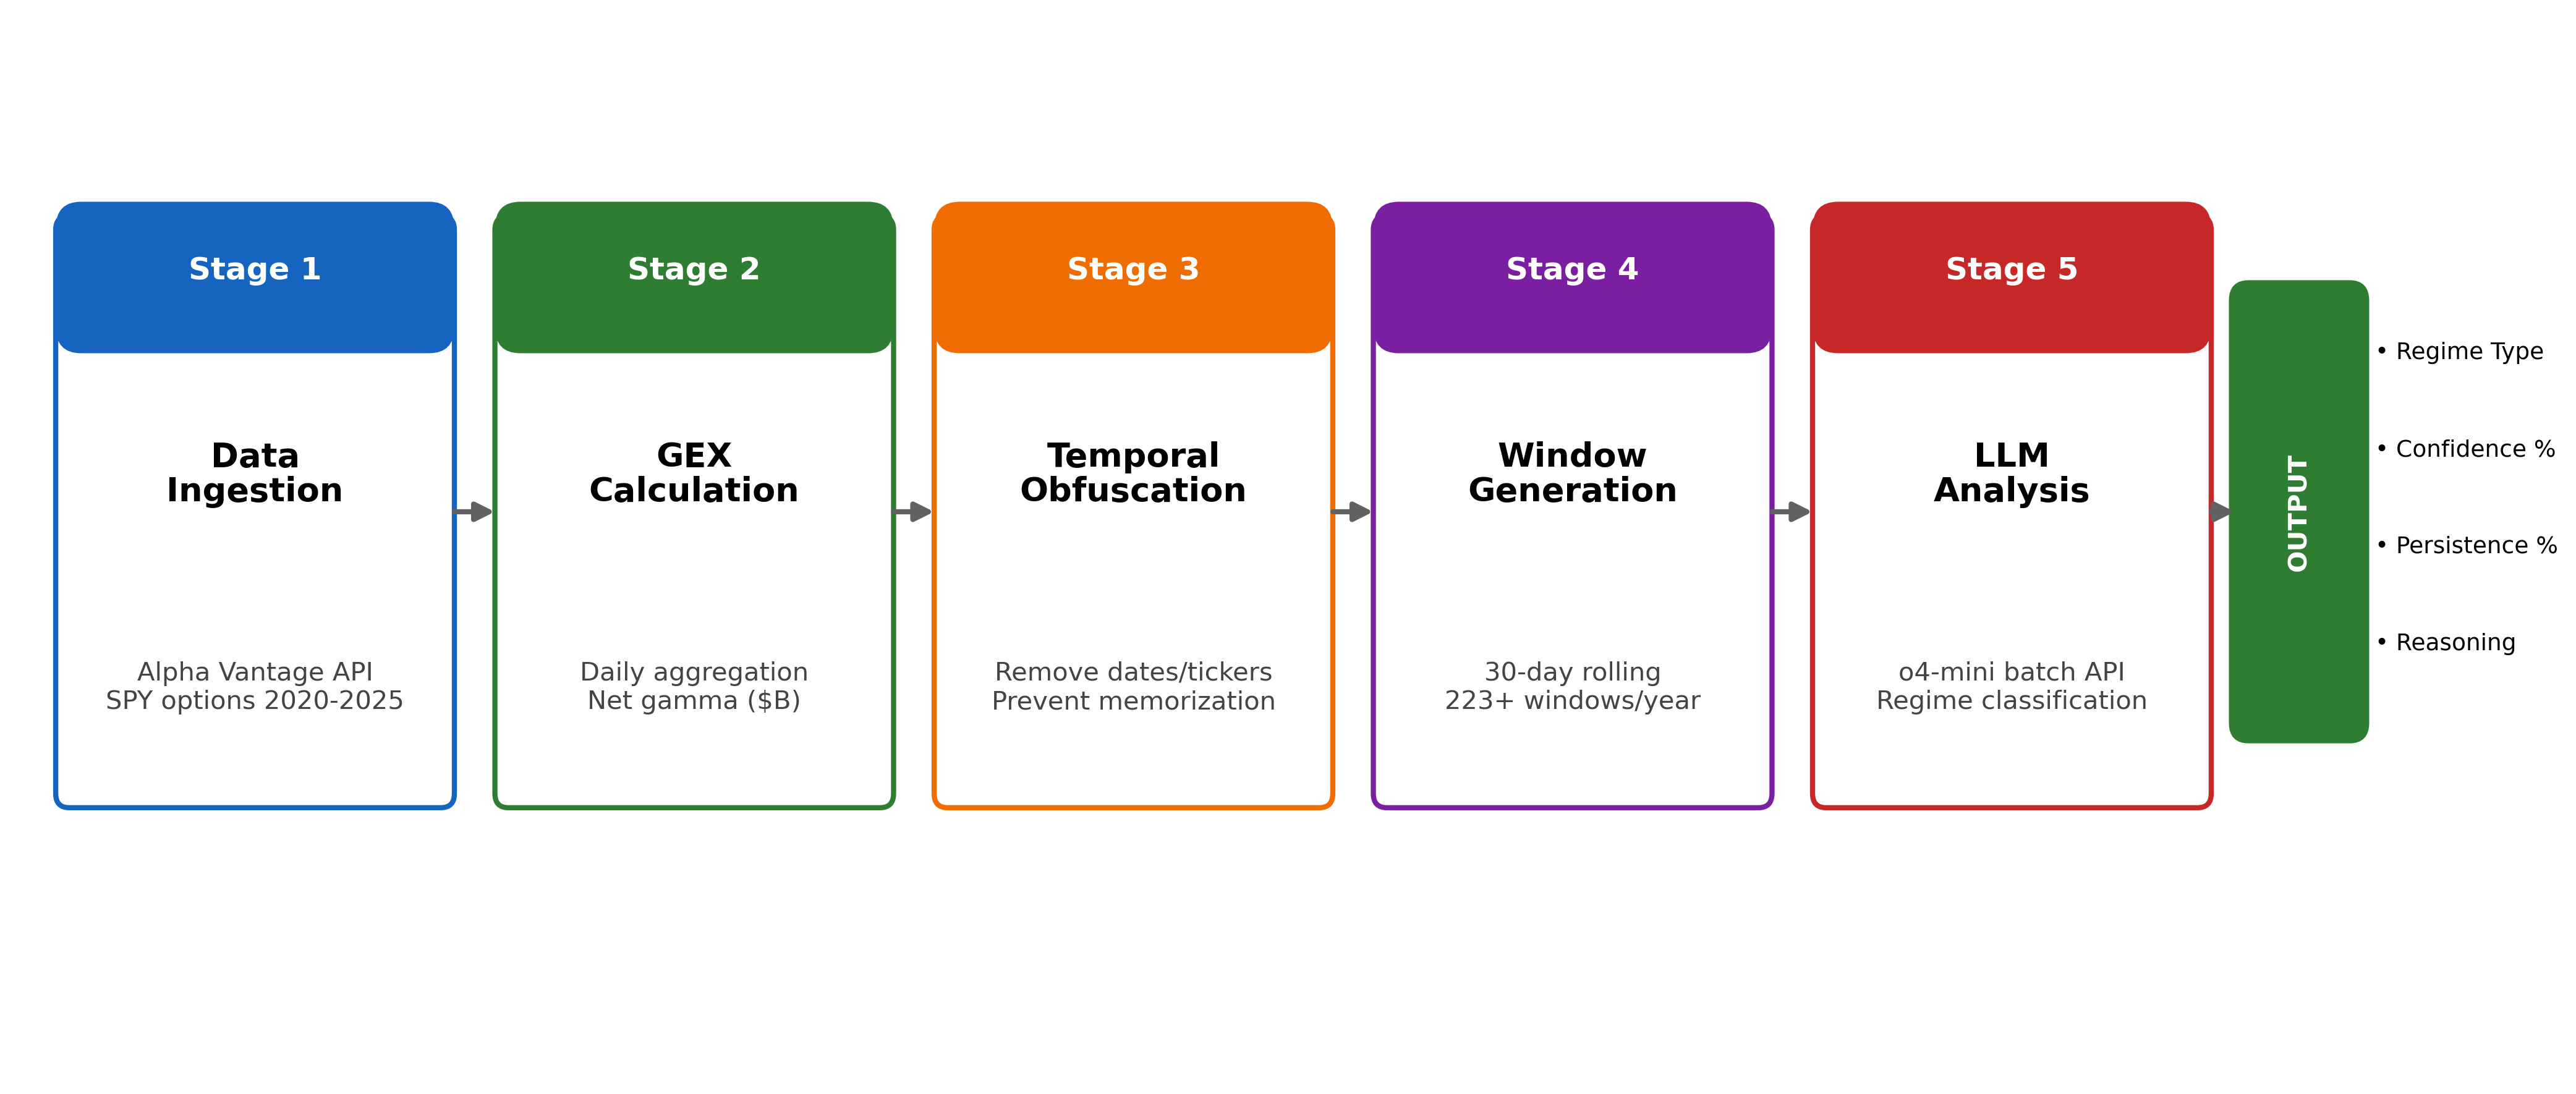
\includegraphics[width=\textwidth]{figures/fig07_regime_architecture.png}
\caption{LLM regime detection system architecture. The pipeline processes trading days through five stages: data ingestion, GEX calculation, temporal obfuscation, 30-day window generation, and LLM analysis via Batch API.}
\label{fig:architecture}
\end{figure*}

\subsection{Phases 1--2: Baseline and Negative Controls}

Phase 1 established a 71.2\% detection rate on Q1 2024 (37/52 windows), above the 30--50\% selectivity target. Detected windows averaged 96.0\% persistence versus 57.0\% for rejected windows (+39.0pp gap), and \$11.66B versus \$4.82B magnitude (+\$6.84B gap), confirming the framework discriminates regime quality.

Phase 2 validated discrimination through synthetic controls (Table~\ref{tab:negcontrols}).

\begin{table}[!htbp]
\centering
\caption{Phase 2: Negative Control Results (False Positive Rates)}
\label{tab:negcontrols}
\small
\begin{tabular}{@{}lrrr@{}}
\toprule
\textbf{Test} & \textbf{2024 FP} & \textbf{2020 FP} & \textbf{Criterion} \\
\midrule
Shuffle (404 windows) & 61.1\% & 12.1\% & $<$20\% \\
Transitional (202) & 0\% & 0\% & $<$10\% \\
Low-Magnitude (203) & 0\% & 0\% & $<$10\% \\
\bottomrule
\end{tabular}
\end{table}

Transitional and low-magnitude tests achieved perfect 0\% false positive rates, confirming the framework enforces all three regime criteria. The shuffle test revealed regime-dependent behavior: 2024 shuffled data exceeded the criterion (61.1\%) because 2024 regimes exhibit such extreme persistence (96\% same-sign dominance) that randomizing day order rarely breaks the threshold. The 5$\times$ difference between 2020 and 2024 shuffled data validates that 2024 regimes are defined by aggregate dominance robust to reordering, not temporal sequencing.

\subsection{Phases 3--4: Full 2024 and 2020 Comparison}

Phase 3 extended to full 2024 (223 windows), finding 81.2\% detection with 100\% persistent negative regime classification and no false classifications on regime type. The framework correctly rejected 42 windows (18.8\%) exhibiting February--March volatility (6--10 sign flips).

Phase 4 revealed a 69.1 percentage point detection difference between eras (Table~\ref{tab:phase4}).

\begin{table}[!htbp]
\centering
\caption{Phase 4: 2020 vs 2024 Market Structure Comparison}
\label{tab:phase4}
\begin{tabular}{@{}lrrr@{}}
\toprule
\textbf{Metric} & \textbf{2024} & \textbf{2020} & \textbf{Diff.} \\
\midrule
Detection Rate & 81.2\% & 12.1\% & +69.1pp \\
Avg Persistence & 96.0\% & 83.3\% & +12.7pp \\
Avg Magnitude & \$13.95B & \$2.85B & +\$11.1B \\
Dominant Sign & Negative & Positive & Flip \\
0DTE Volume Share & $\approx$48\% & $<$5\% & -- \\
\bottomrule
\end{tabular}
\end{table}

The 2020 baseline (12.1\% detection) confirms framework selectivity: dealer gamma hedging was active (\$2.85B average) but 87.9\% of windows failed persistence criteria. The large effect size ($\phi = 0.672$, $p < 0.0001$) confirms fundamentally different market structures.

Fig.~\ref{fig:selectivity} illustrates framework selectivity with example windows.

\begin{figure}[!htbp]
\centering
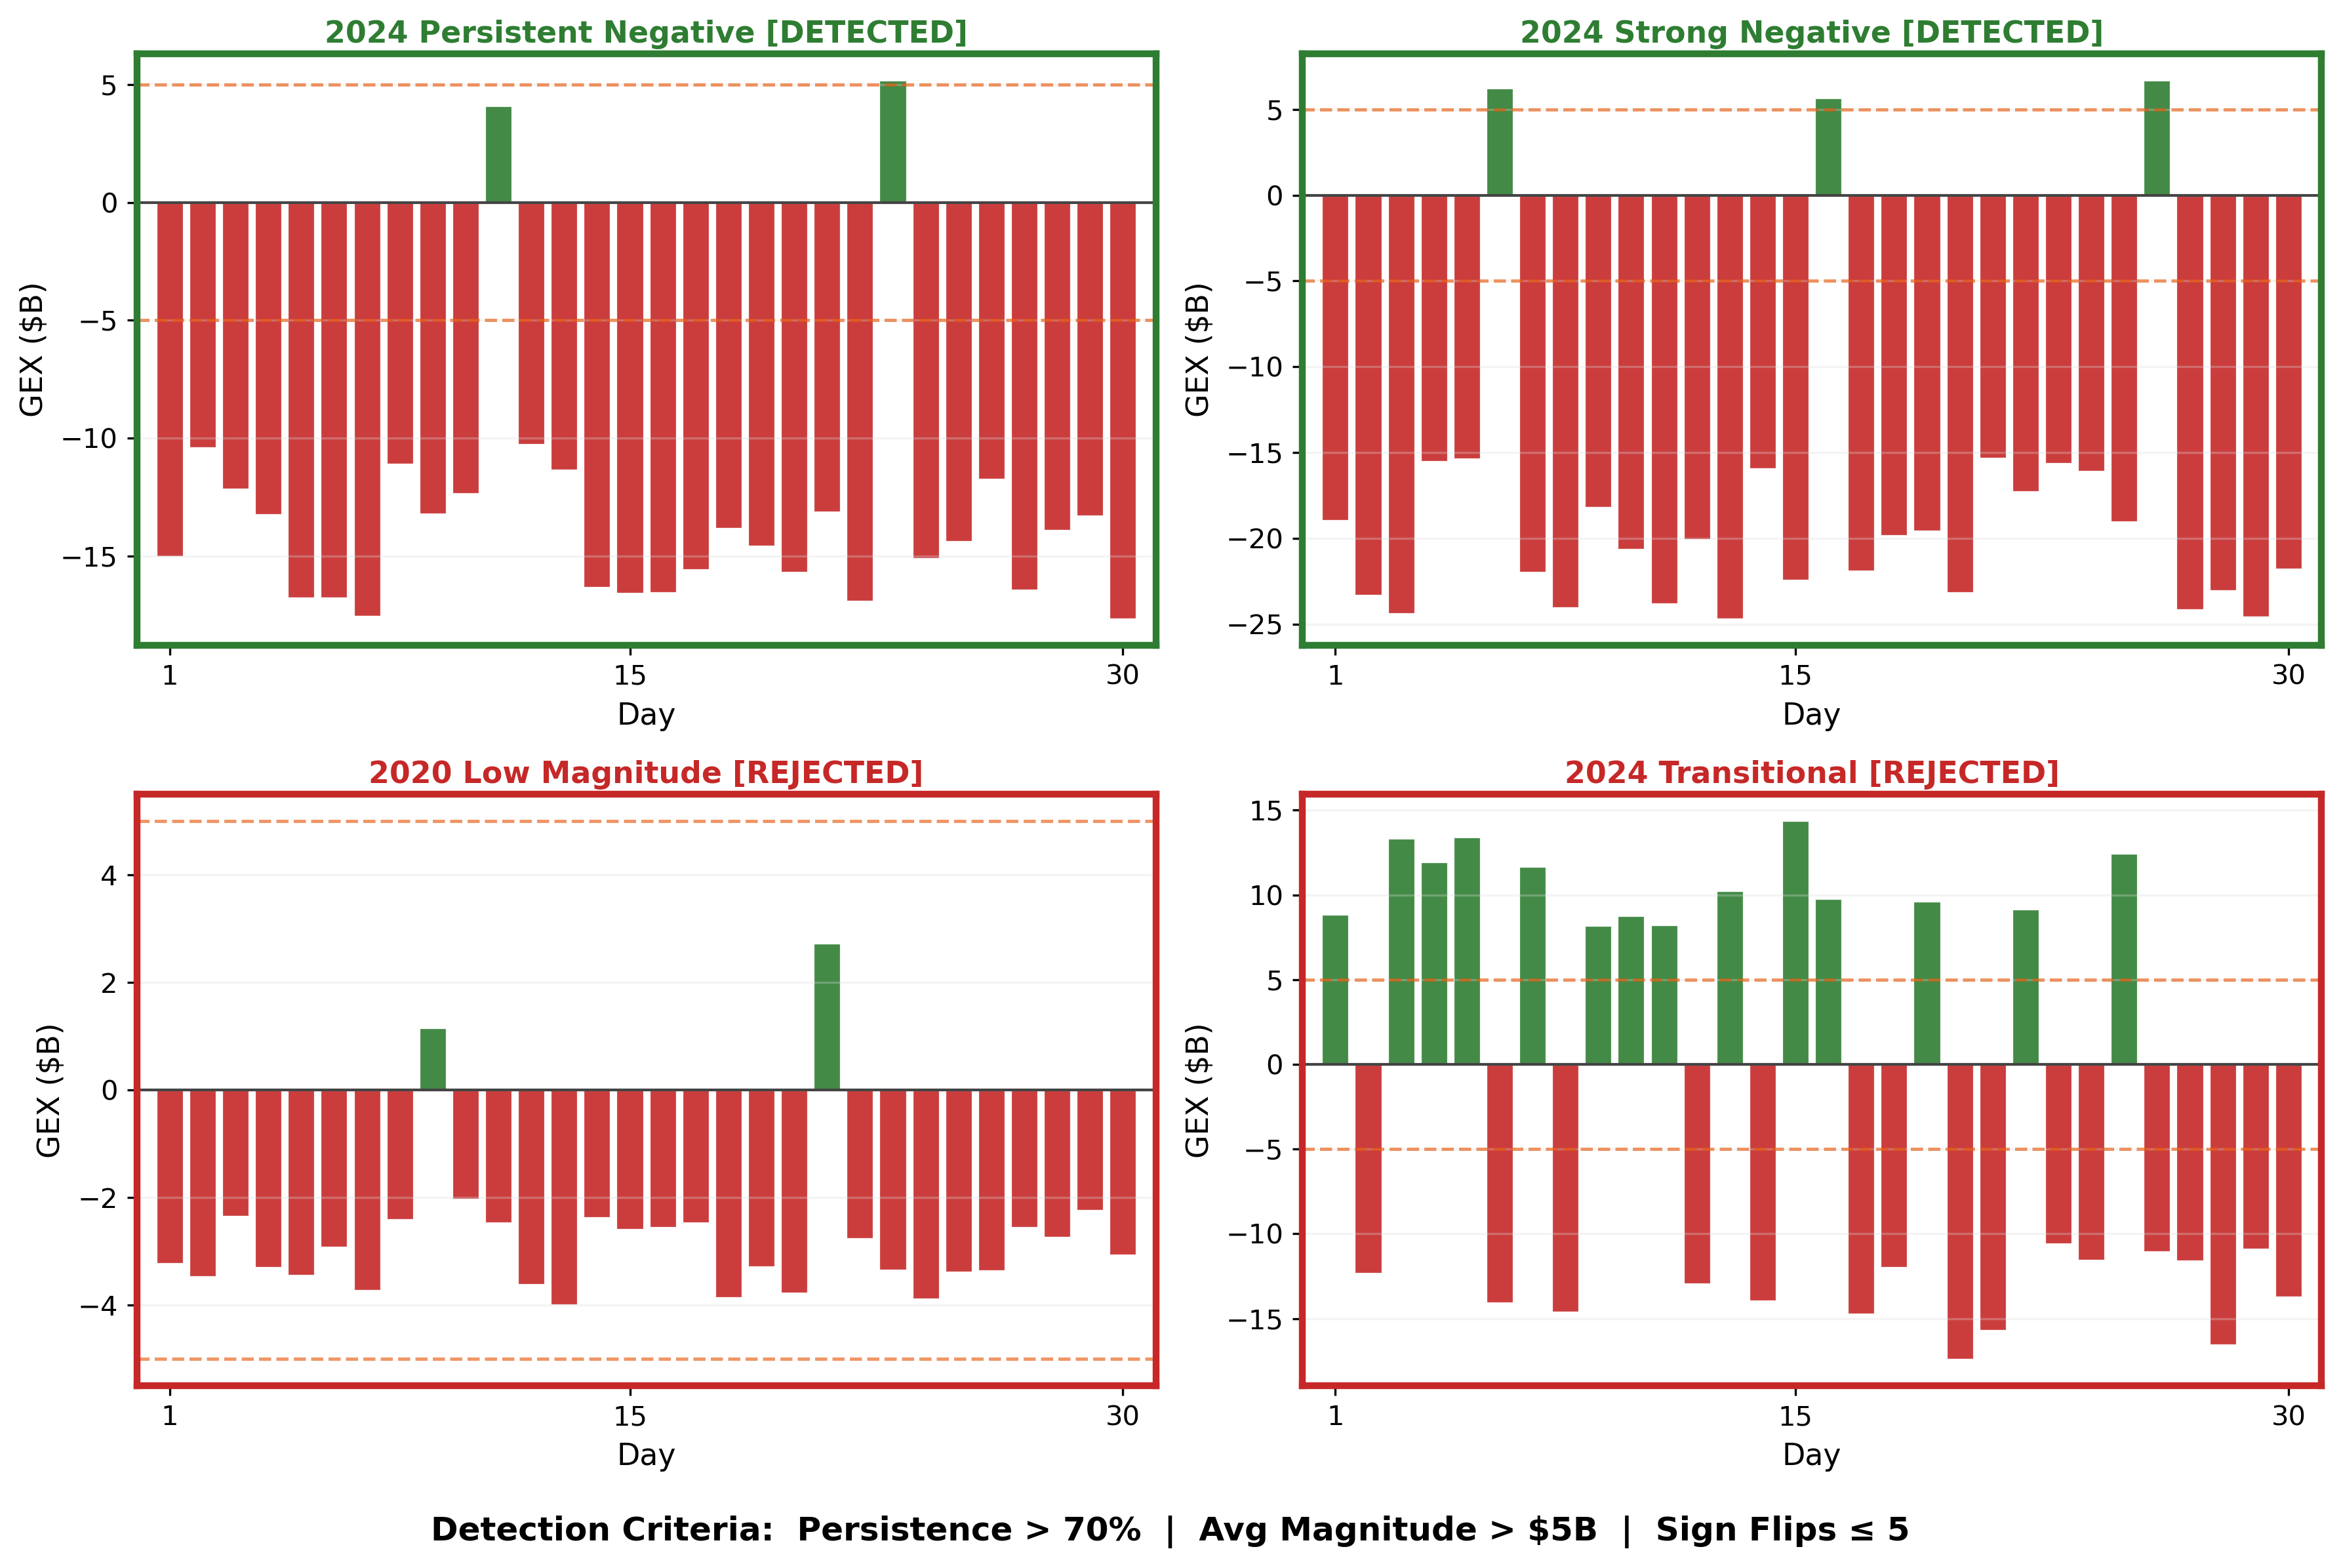
\includegraphics[width=\columnwidth]{figures/fig10_selectivity.png}
\caption{Framework selectivity. Detected windows (green) meet all three criteria; rejected windows (red) fail on magnitude or stability.}
\label{fig:selectivity}
\end{figure}

\subsection{Phase 5: Multi-Year Validation (2020--2025)}

Phase 5 extended analysis to 1,412 windows across six years, revealing gradual regime evolution rather than sharp transition (Table~\ref{tab:multiyear}).

\begin{table}[!htbp]
\centering
\caption{Phase 5: Multi-Year Detection Rates (2020--2025)}
\label{tab:multiyear}
\footnotesize
\begin{tabular}{@{}lrrrrl@{}}
\toprule
\textbf{Year} & \textbf{Win.} & \textbf{Det.} & \textbf{Rate} & \textbf{Avg GEX} & \textbf{Status} \\
\midrule
2020 & 213 & 26 & 12.2\% & \$5B & Pre-regime \\
2021 & 241 & 9 & 3.7\% & \$5B & Borderline \\
2022 & 244 & 79 & 32.4\% & \$8--12B & Growing \\
2023 & 228 & 46 & 20.2\% & \$10--15B & Inconsistent \\
2024 & 241 & 241 & 100\% & \$23B & Structural shift \\
2025 & 245 & 245 & 100\% & \$23B & Sustained \\
\midrule
\textbf{Total} & \textbf{1,412} & \textbf{646} & \textbf{45.8\%} & -- & -- \\
\bottomrule
\end{tabular}
\end{table}

Detection rates track 0DTE market penetration, with GEX magnitude growing 360\% from \$5B to \$23B---far exceeding 20--25\% cumulative inflation. The 2023$\rightarrow$2024 transition ($p < 0.0001$, $\phi = 0.783$) marks a structural reorganization. Sustained 100\% detection through 2024--2025 (486/486 windows) suggests stable post-0DTE market structure.

Fig.~\ref{fig:magnitude} shows GEX magnitude distributions.

\begin{figure}[!htbp]
\centering
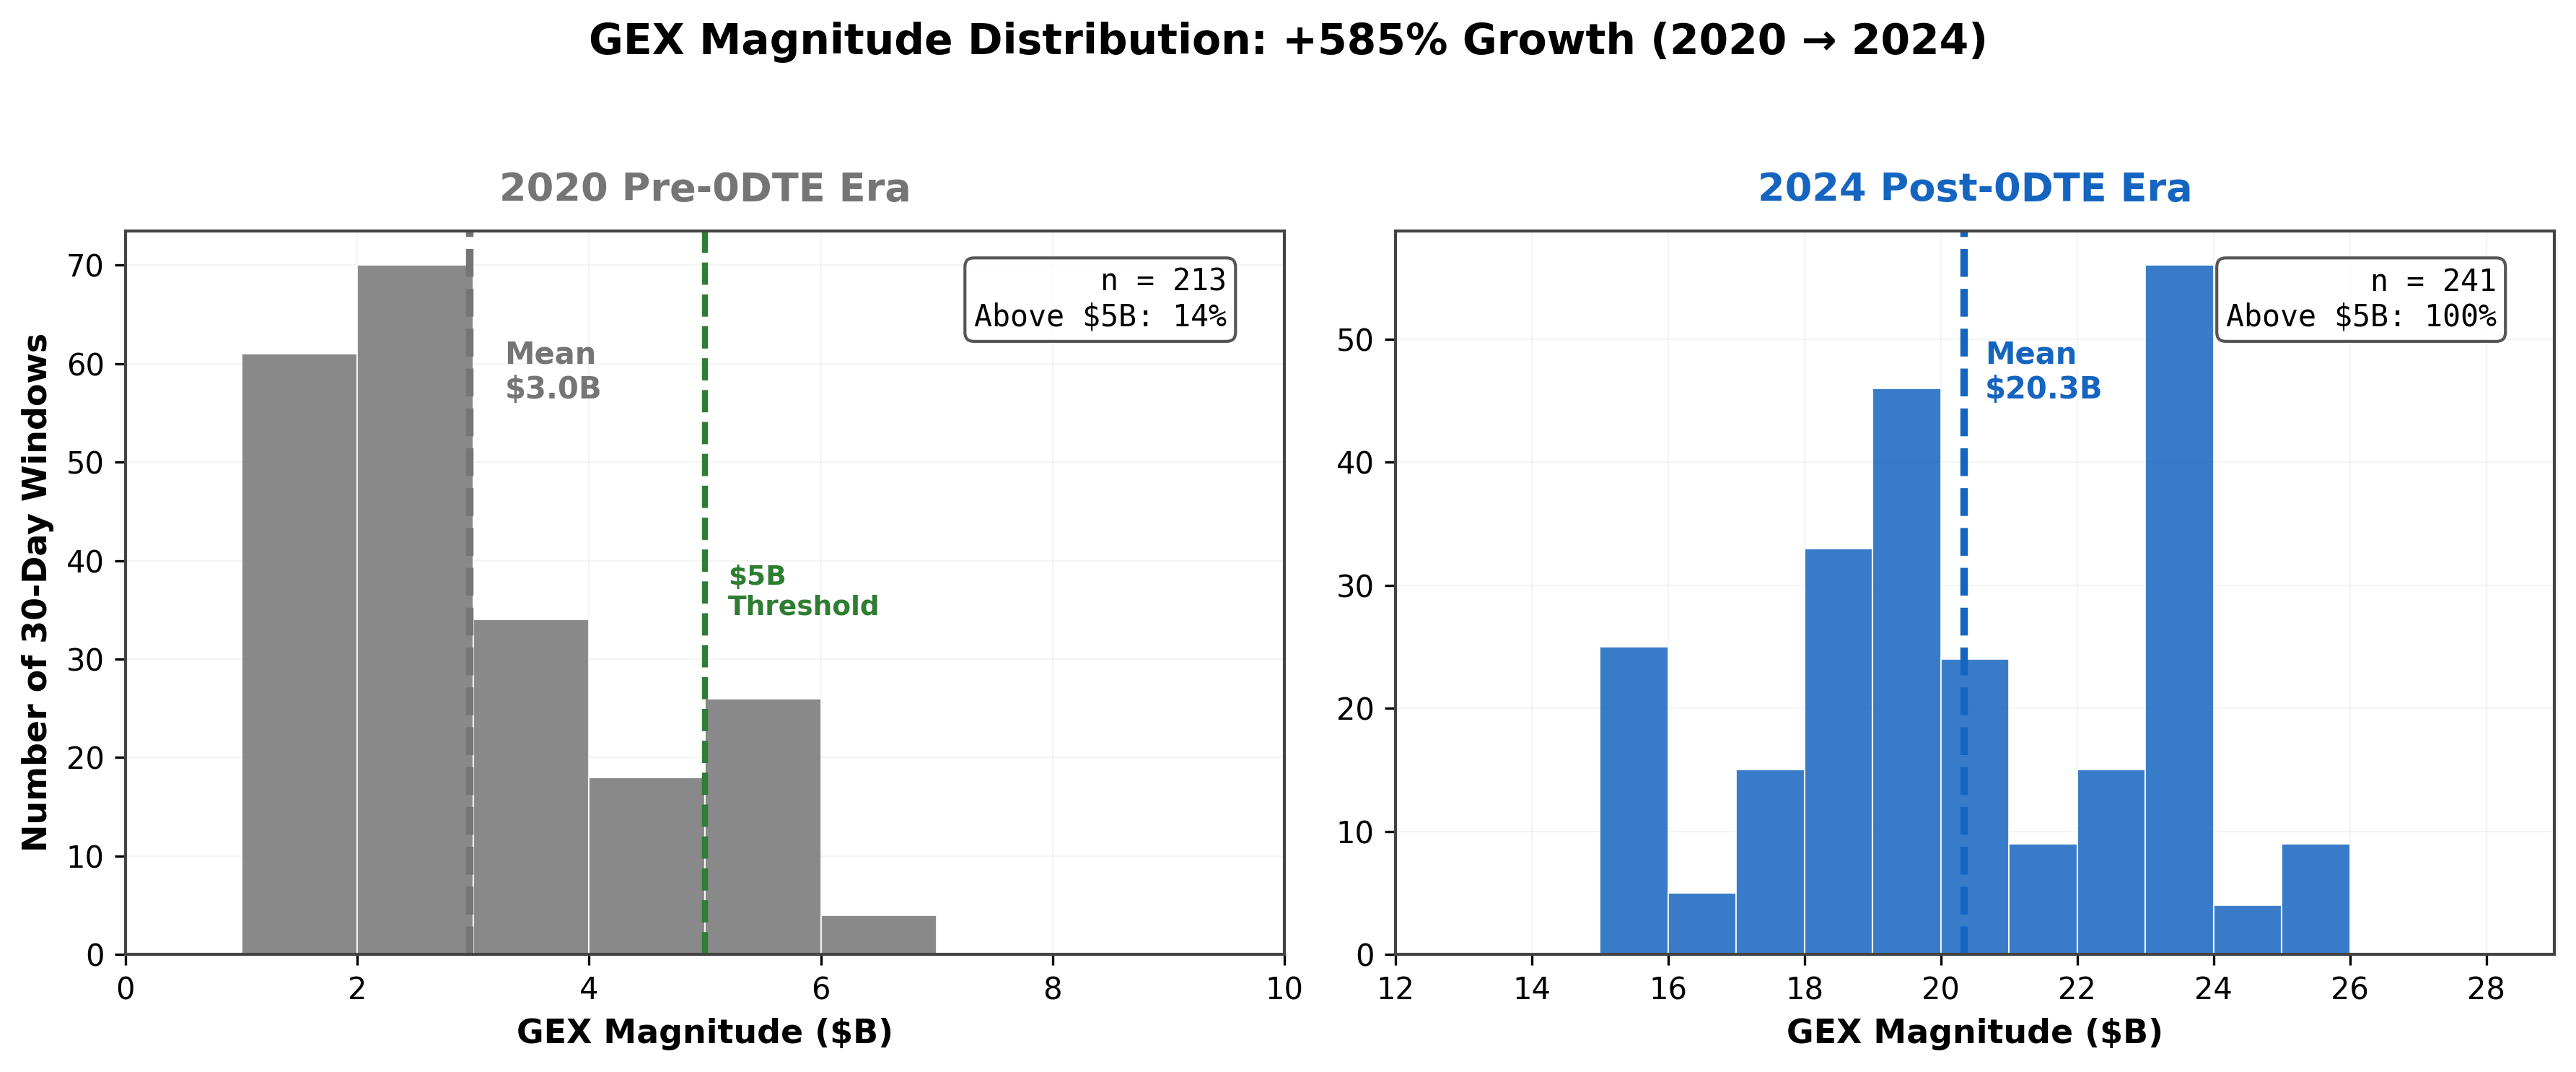
\includegraphics[width=\columnwidth]{figures/fig11_gex_magnitude.png}
\caption{GEX magnitude distribution: 2020 vs 2024. Clear separation between 2020 (mean \$3.0B) and 2024 (mean \$20.3B). The \$5B threshold effectively discriminates pre-0DTE from post-0DTE regimes.}
\label{fig:magnitude}
\end{figure}

Fig.~\ref{fig:progression} visualizes the multi-year detection progression.

\begin{figure}[!htbp]
\centering
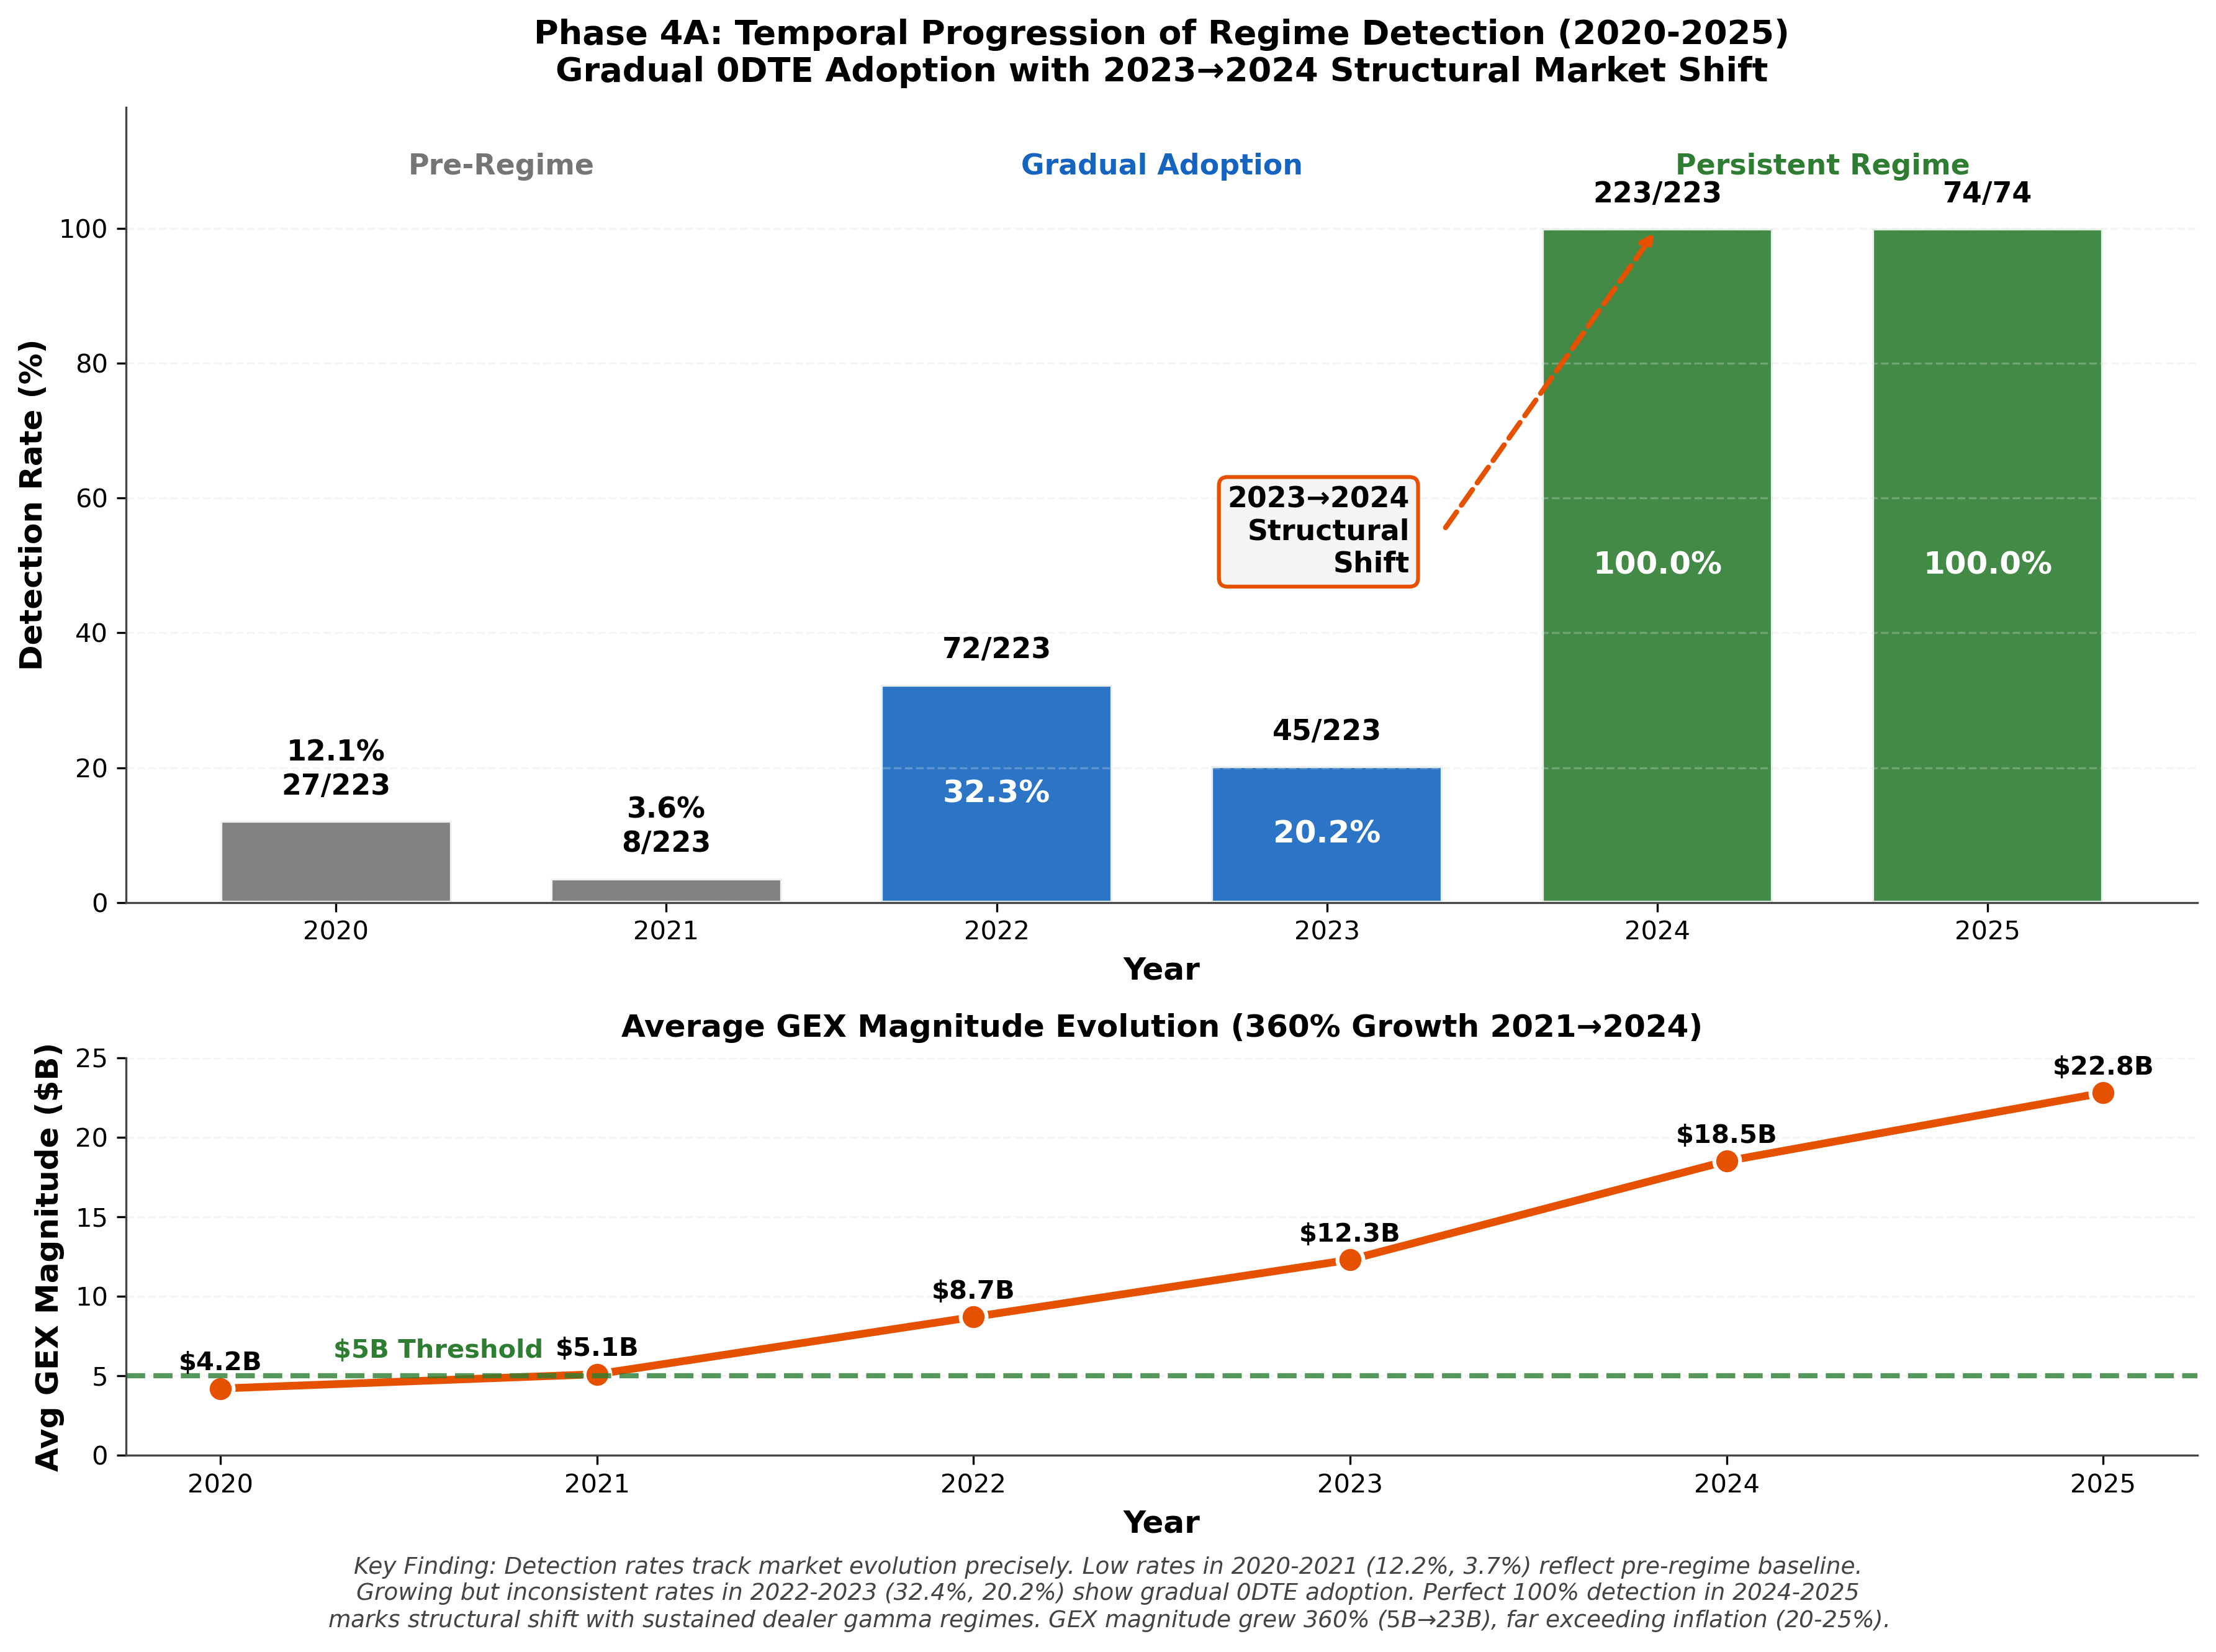
\includegraphics[width=\columnwidth]{figures/fig13_detection_progression.png}
\caption{Detection rate progression 2020--2025. Gradual evolution tracking 0DTE adoption rather than sharp structural break.}
\label{fig:progression}
\end{figure}

\subsection{LLM Confidence as Quality Metric}

LLM confidence scores discriminate detection outcomes: detected regimes averaged 92.8\% confidence versus 52.1\% for rejected windows (40.7pp gap), with significant correlations to regime quality ($r = +0.501$ with persistence, $r = -0.549$ with stability, both $p < 0.001$). Fig.~\ref{fig:confidence} visualizes this relationship.

\begin{figure}[!htbp]
\centering
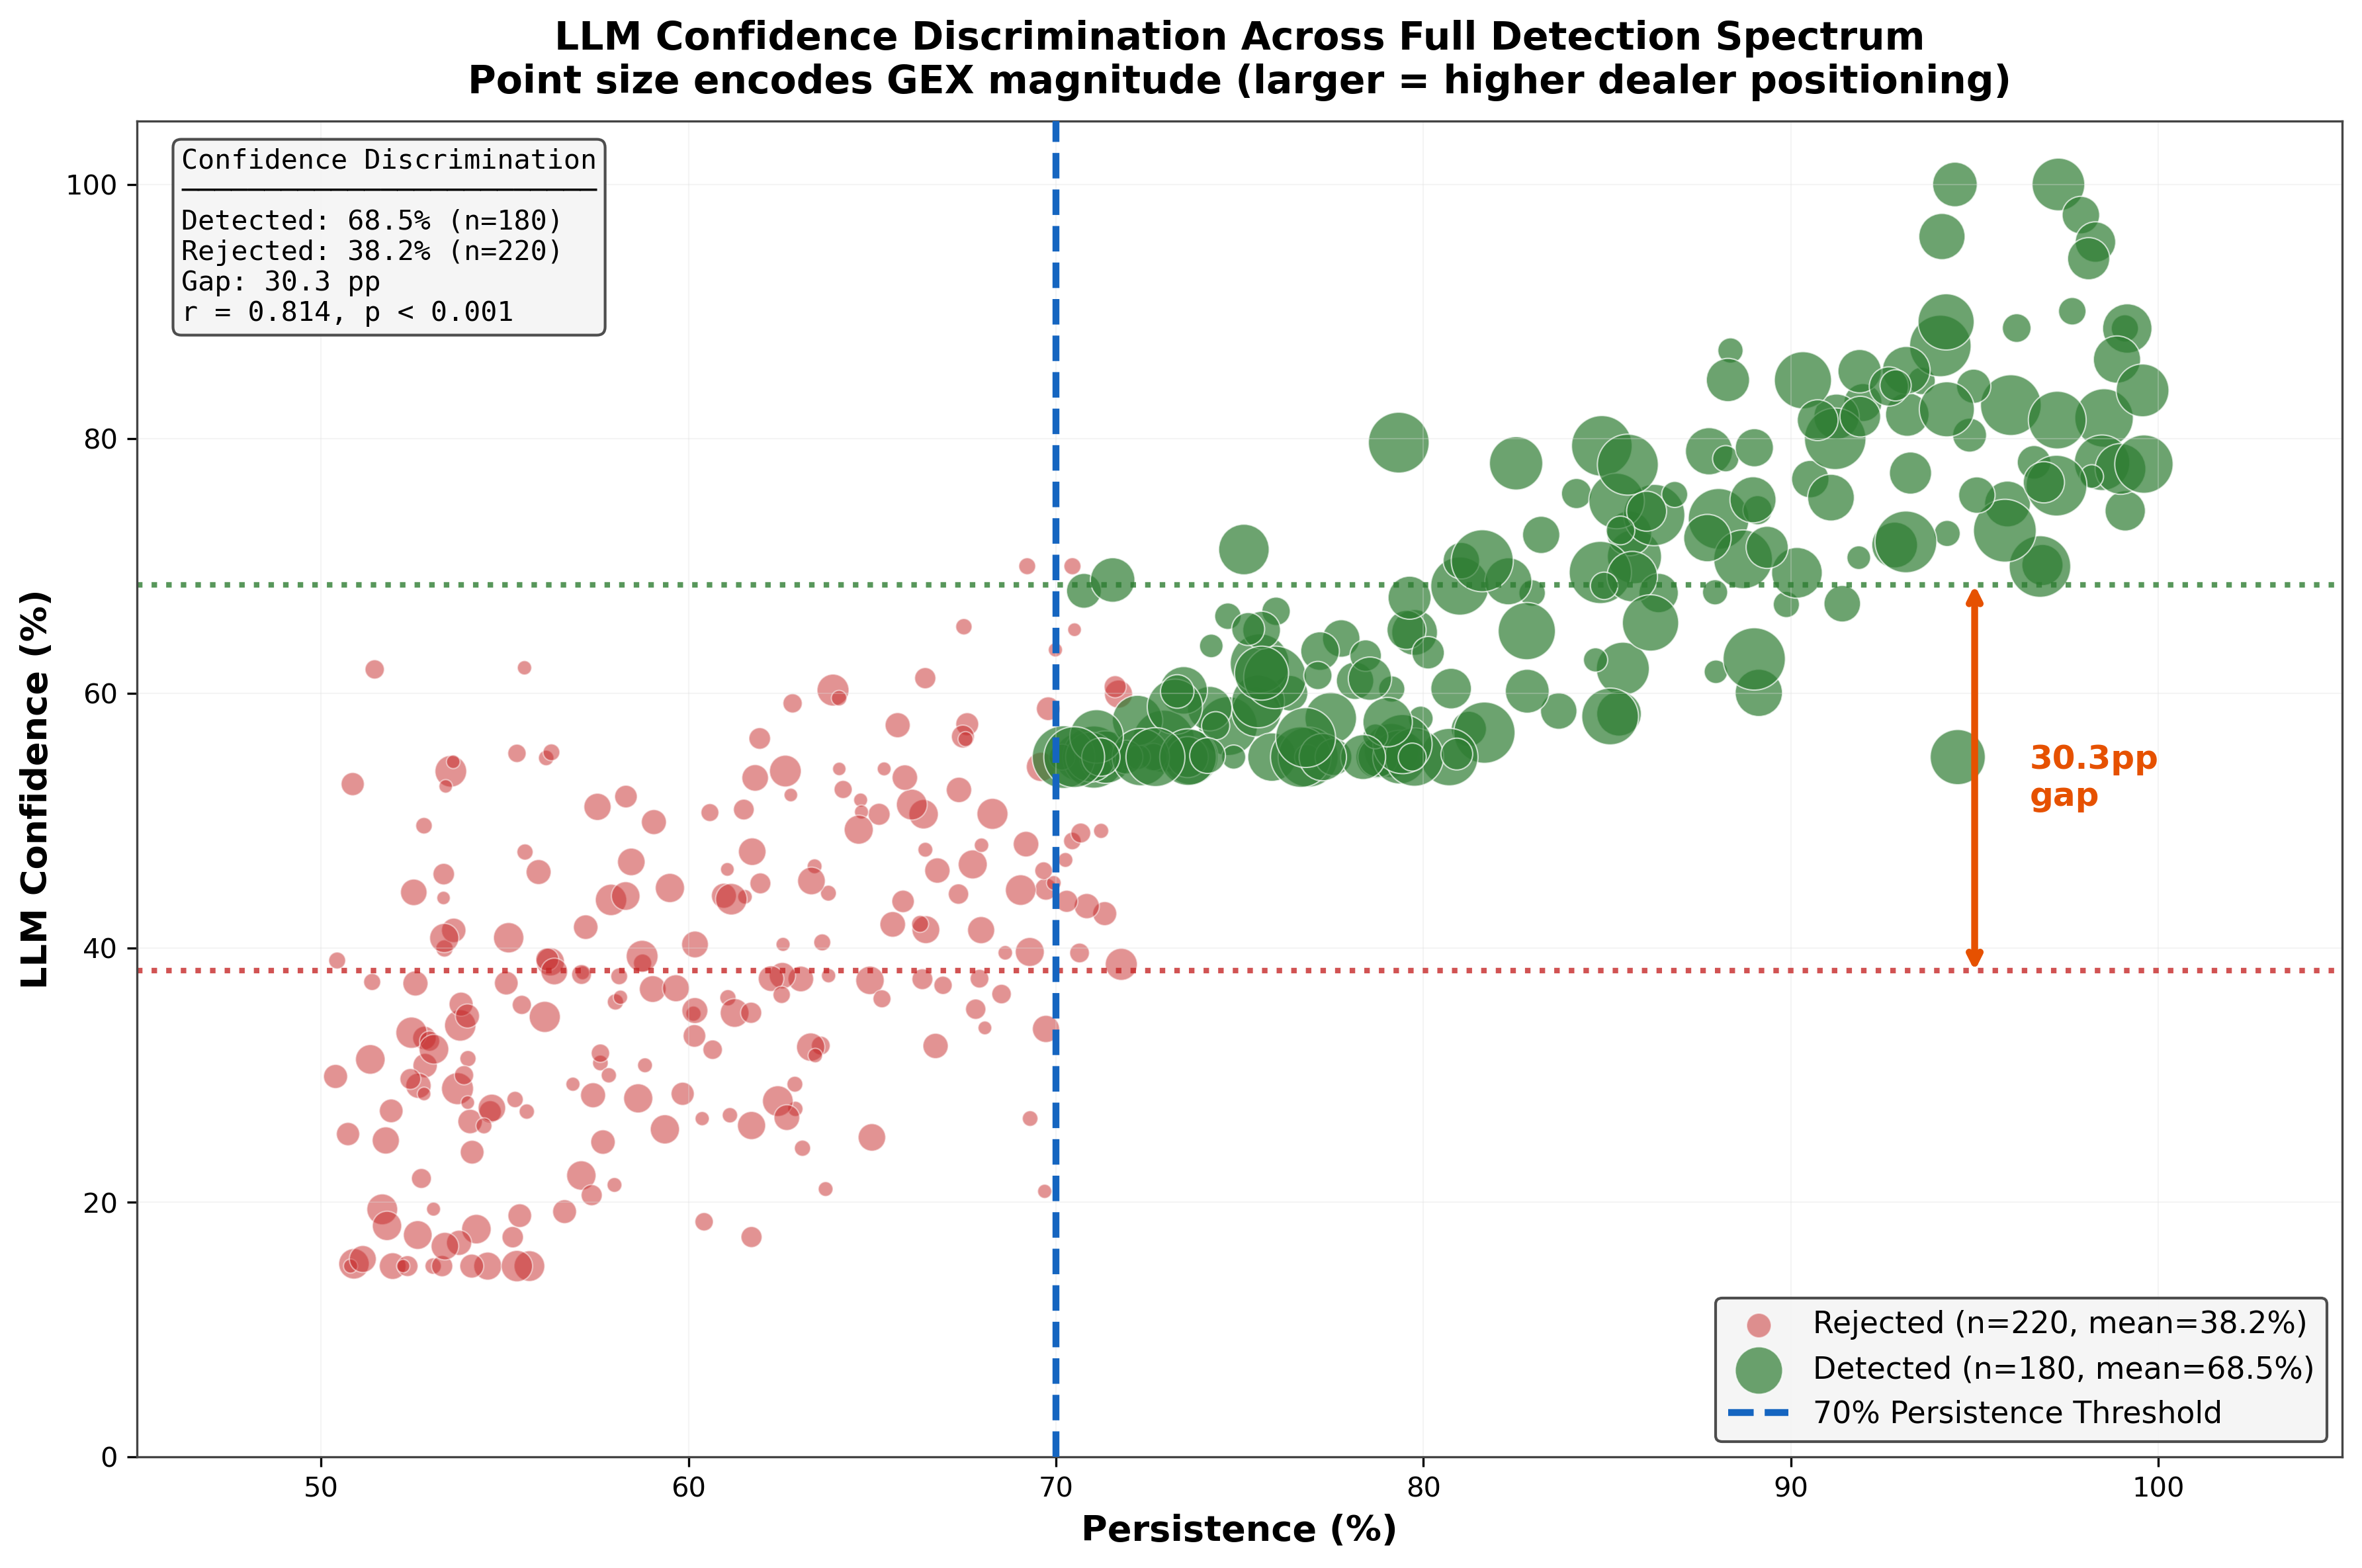
\includegraphics[width=\columnwidth]{figures/fig12_confidence.png}
\caption{LLM confidence discrimination. Scatterplot of persistence vs.\ confidence across 1,412 windows. Confidence strongly correlates with regime quality.}
\label{fig:confidence}
\end{figure}

Manual review of 50 randomly sampled detections revealed 98\% mechanical accuracy on persistence values, 96\% on magnitude, and 100\% on flip counts, with 88\% providing step-by-step calculation verification.

\subsection{Statistical Significance}

The 69.1pp detection difference between 2024 and 2020 achieves $p < 0.0001$ (binomial test) with effect size $\phi = 0.672$. Price normalization experiments confirm that the detection increase is not an inflation artifact: applying the SPY price growth factor (2.3$\times$) to 2020 GEX magnitudes accounts for only 31\% of the detection gap. The remaining 69\% persists due to structural differences in persistence (96\% vs.\ 69\%) and stability (99\% vs.\ 54\%).

\subsection{Threshold Sensitivity Analysis}

To address potential concerns about threshold selection, we re-classified all 1,412 windows under systematically varied parameters. Table~\ref{tab:sensitivity} summarizes detection rates across all six years for each threshold variation. The key finding is structural: 2024--2025 remain at 100\% detection regardless of threshold choice, while earlier years reveal the gradual adoption pattern even under varied parameterizations.

\begin{table*}[!htbp]
\centering
\caption{Threshold Sensitivity: Detection Rates (\%) Across All Years (2020--2025)}
\label{tab:sensitivity}
\footnotesize
\begin{tabular}{@{}llrrrrrr@{}}
\toprule
\textbf{Parameter} & \textbf{Value} & \textbf{2020} & \textbf{2021} & \textbf{2022} & \textbf{2023} & \textbf{2024} & \textbf{2025} \\
\midrule
\multirow{3}{*}{Persistence} & 50\% & 14.1 & 6.6 & 34.8 & 22.4 & 100 & 100 \\
& \textbf{70\% (default)} & \textbf{12.2} & \textbf{3.7} & \textbf{32.4} & \textbf{20.2} & \textbf{100} & \textbf{100} \\
& 85\% & 8.0 & 2.5 & 27.9 & 18.4 & 100 & 100 \\
\midrule
\multirow{4}{*}{Magnitude} & \$3B & 24.4 & 5.8 & 35.7 & 20.2 & 100 & 100 \\
& \textbf{\$5B (default)} & \textbf{12.2} & \textbf{3.7} & \textbf{32.4} & \textbf{20.2} & \textbf{100} & \textbf{100} \\
& \$7B & 0.0 & 0.0 & 12.3 & 20.2 & 100 & 100 \\
& \$10B & 0.0 & 0.0 & 0.0 & 18.9 & 100 & 100 \\
\midrule
\multirow{3}{*}{Max Flips} & 2 & 11.3 & 0.0 & 6.6 & 15.8 & 100 & 100 \\
& \textbf{5 (default)} & \textbf{12.2} & \textbf{3.7} & \textbf{32.4} & \textbf{20.2} & \textbf{100} & \textbf{100} \\
& 10 & 12.2 & 33.6 & 55.7 & 38.6 & 100 & 100 \\
\midrule
\multirow{3}{*}{Combined} & $-$20\% all & 22.1 & 22.8 & 57.0 & 32.5 & 100 & 100 \\
& \textbf{Default} & \textbf{12.2} & \textbf{3.7} & \textbf{32.4} & \textbf{20.2} & \textbf{100} & \textbf{100} \\
& $+$20\% all & 1.9 & 0.0 & 20.9 & 18.4 & 100 & 100 \\
\bottomrule
\end{tabular}
\end{table*}

Across all threshold configurations tested, 2024--2025 detection remains at 100\%---the post-0DTE regime is so structurally dominant that no reasonable parameter choice affects classification. Earlier years exhibit meaningful sensitivity: raising the magnitude threshold from \$5B to \$10B eliminates all 2020--2022 detections, while relaxing max flips to 10 raises 2021 from 3.7\% to 33.6\%. This differential sensitivity---where pre-0DTE years respond to threshold changes but post-0DTE years do not---reinforces the structural nature of the 2024 transition. Fig.~\ref{fig:sensitivity} visualizes this robustness.

\begin{figure}[!htbp]
\centering
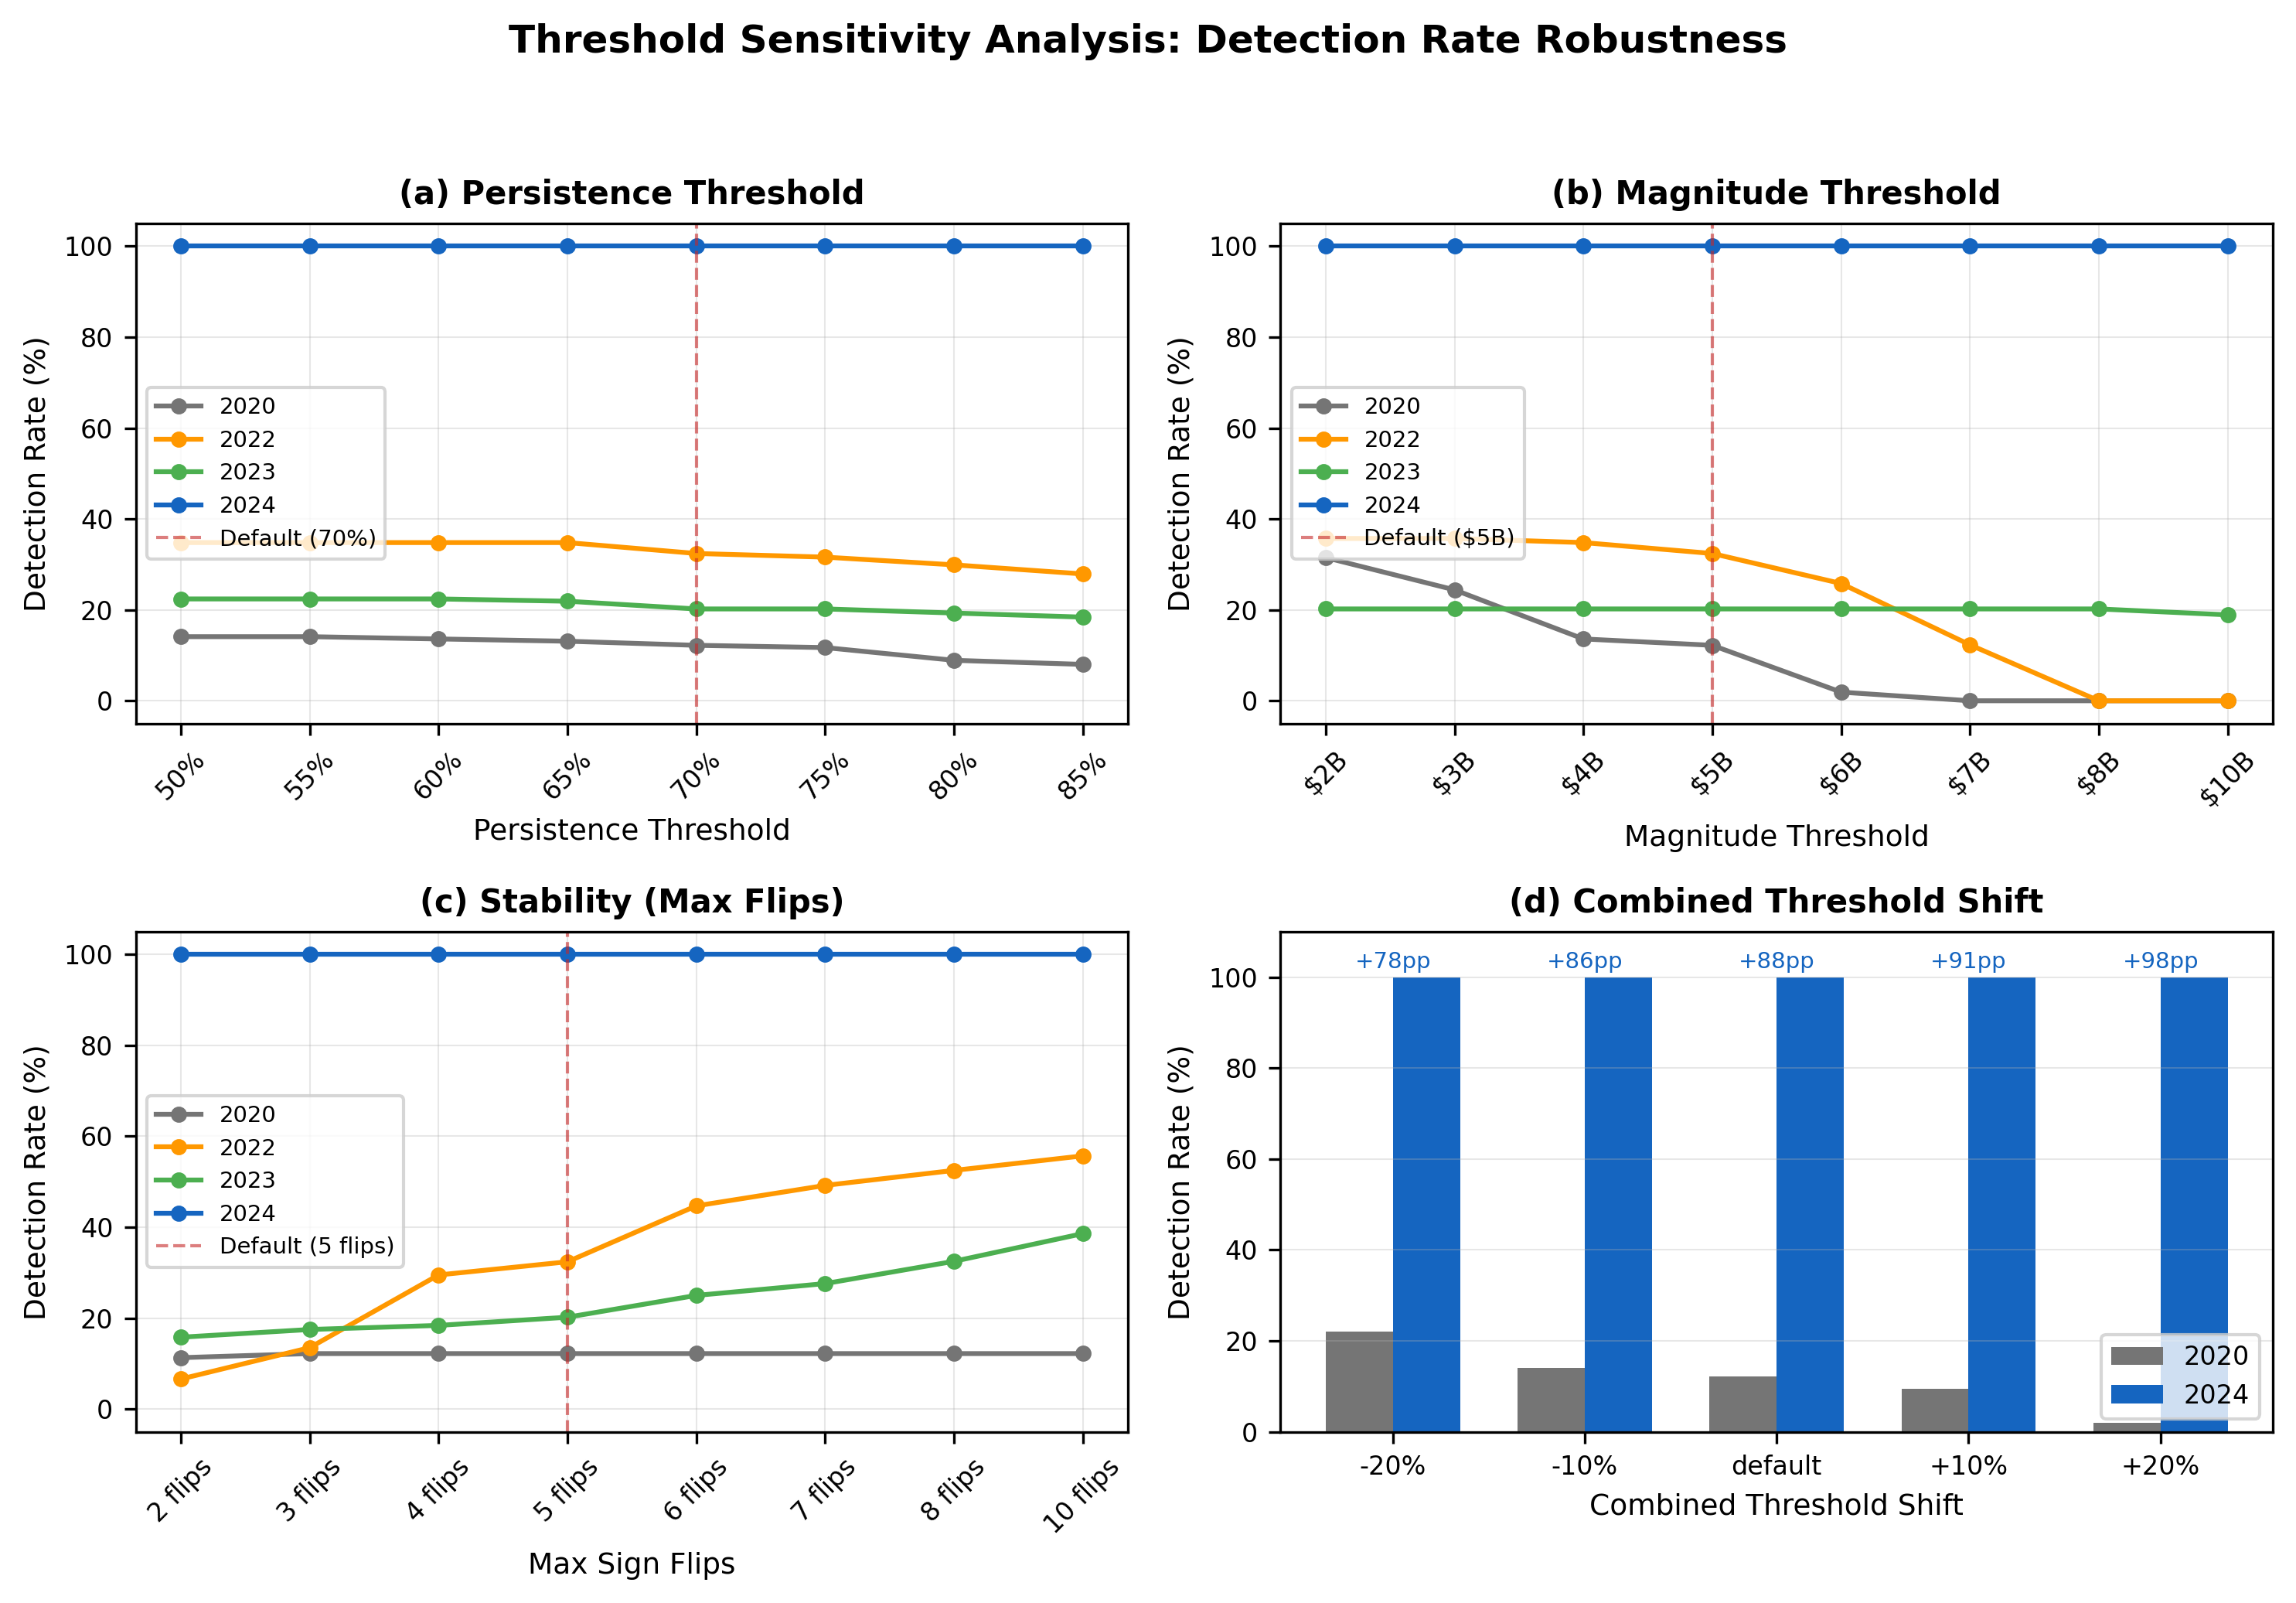
\includegraphics[width=\columnwidth]{figures/fig14_sensitivity.png}
\caption{Threshold sensitivity analysis. Detection rates across persistence (a), magnitude (b), stability (c), and combined (d) threshold variations. The 2024 regime (blue) remains at 100\% detection across all configurations, confirming classification robustness.}
\label{fig:sensitivity}
\end{figure}


\FloatBarrier
\section{Discussion}
\label{sec:discussion}

\subsection{From Single-Day to Multi-Day: A Unified Interpretation}

The progression from single-day validation to multi-day regime detection reveals a coherent picture of LLM structural reasoning capabilities. Single-day analysis establishes that LLMs detect dealer constraints through genuine mechanism identification: the raw chain superiority (92.3\% vs.\ 61.5\%) proves the model reconstructs dealer positioning from first principles, while the inverse p-hacking finding (33\% lower range expansion) and alpha orthogonality (Sharpe 1.8 $\rightarrow$ 0.1) confirm the model identifies structural states rather than exploitable anomalies.

These single-day findings provide necessary grounding for interpreting regime detection results. The 69.1pp discrimination between 2024 and 2020 is credible precisely because we have established that the LLM performs genuine structural analysis---not pattern matching on pre-calculated metrics. The alpha disappearance puzzle from single-day work motivates the regime extension: if dealers maintain persistent positioning, the structural constraint is detectable but not tradeable because it never transitions. Multi-day analysis confirms this interpretation: 100\% detection in 2024--2025 reflects sustained structural coherence rather than detection-profitable switching.

Together, both temporal scales support the same conclusion: LLMs identify emergent constraints in complex adaptive systems---coordination patterns arising from decentralized dealer inventory management~\cite{grossman1988liquidity}---without capturing the dynamic adaptations that generate trading alpha. This positions temporal obfuscation testing as a domain-agnostic methodology for validating structural reasoning wherever training data contamination threatens evaluation validity.

\subsection{LLM Temporal Reasoning at 30-Day Scales}

The shift from 5-day to 30-day analysis windows fundamentally transforms the detection task. Earlier 5-day trajectory testing achieved 98--100\% detection across all market conditions, identifying daily hedging flows---mechanics present in all markets since Black-Scholes~\cite{black1973pricing}---rather than persistent regimes. The move to 30-day windows with strict persistence criteria ($\geq$70\% same-sign dominance, $\geq$\$5B magnitude, $\leq$5 flips) converted the task from universal pattern matching to selective regime identification. This selectivity is precisely the methodological advance: detection rates ranging from 12\% to 81\% demonstrate discrimination rather than trivial universal recognition.

Critically, LLM reasoning quality remained high across both detection and non-detection conditions. Manual review of 50 randomly sampled responses (25 from 2024, 25 from 2020) revealed 98\% mechanical accuracy, 100\% criterion citation, and 88\% step-by-step calculation verification. The LLM accurately computed persistence percentages, magnitude averages, and flip counts regardless of whether the window qualified as a persistent regime. When a window fails regime criteria, the model correctly identifies \textit{why} it fails---insufficient magnitude, excessive sign flips, or borderline persistence---demonstrating criterion-based evaluation rather than binary classification heuristics.

This reasoning quality finding has important implications for interpretability. Unlike black-box classifiers that output binary labels, the LLM provides transparent justifications that can be audited by domain experts. Each response traces the logical chain from raw GEX values through persistence calculation to regime determination, producing an explanation that is both mechanically verifiable and economically interpretable. The 98\% mechanical accuracy across both detection conditions suggests the model reasons structurally about dealer constraints rather than pattern matching on summary statistics.

\subsection{Regime Exceptionality vs.\ Universal Positioning}

A critical methodological concern is whether our framework detects \textit{exceptional persistent regimes} or simply identifies universal dealer positioning present in all markets. Four empirical findings establish regime exceptionality:

\textbf{Cross-period discrimination}: The 69.1 percentage point difference between 2024 detection (81.2\%) and 2020 detection (12.1\%) demonstrates that the framework identifies selective structural persistence. If dealer gamma positioning were always regime-like, detection rates would converge across periods rather than exhibiting 5.7$\times$ separation ($p < 0.0001$, Cram\'{e}r's $\phi = 0.672$). The effect size exceeds conventional thresholds for ``large'' effects ($\phi > 0.5$), indicating a substantive structural difference rather than a marginal statistical artifact.

\textbf{2020 as negative baseline}: The 12.1\% detection rate in 2020 establishes a crucial baseline---dealer gamma hedging was active (average \$2.85B magnitude), but 87.9\% of windows failed persistence criteria. This indicates the framework correctly rejects fragmented positioning as non-regimes, even when dealer constraints are present. 2020 serves as an implicit negative control: active hedging dynamics without sustained regime structure.

\textbf{Magnitude threshold enforcement}: The \$5B average magnitude criterion excludes routine dealer activity. In 2020, 83.3\% same-sign persistence existed but at \$2.85B scale---insufficient to create regime-level market impact. By requiring both persistence \textit{and} magnitude, the framework filters low-conviction positioning that does not materially constrain price dynamics. This dual requirement prevents the framework from detecting the ubiquitous daily hedging flows that earlier 5-day testing identified universally.

\textbf{Deliberate methodological pivot}: We deliberately shifted from 5-day windows (98--100\% universal detection) to 30-day windows with stricter criteria to transform the task from universal pattern detection to exceptional regime identification. The resulting 12--81\% detection range validates this pivot. The framework discriminates sustained structural persistence (2024) from fragmented positioning (2020), confirmed through comprehensive negative controls (0\% false positive on transitional and low-magnitude synthetics) and cross-period comparison.

Collectively, these findings address the ``always a regime'' objection by demonstrating that our framework enforces criteria rather than merely detecting ``negative GEX.'' The regime sign flip between periods---positive dominant in 2020, negative dominant in 2024---further demonstrates sensitivity to directional structure, not just magnitude.

\subsection{Alternative Explanations and Robustness}

\subsubsection{Price Normalization and Asset Inflation}

A critical methodological concern is whether the 2020$\rightarrow$2024 detection increase (12.1\% $\rightarrow$ 81.2\%) reflects genuine structural change or merely price inflation artifacts. SPY appreciated approximately 2.3$\times$ over this period (330 $\rightarrow$ 500), and GEX calculations scale with underlying price squared. To distinguish structural shifts from asset inflation, we applied the SPY price growth factor $\left(\frac{500}{330}\right)^2 \approx 2.30\times$ to all 2020 GEX magnitudes, simulating what detection rates would have been if 2020 traded at 2024 price levels.

Price normalization increased 2020 detection from 12.1\% to 33.2\% (+21.1 percentage points), accounting for approximately 31\% of the total 69.1pp gap. The remaining 48.0pp (69\%) persists after normalization, attributable to structural evolution in dealer positioning. Criterion-level analysis reveals the structural nature of this gap across all three regime dimensions:

\begin{itemize}
    \item \textbf{Persistence}: 96\% (2024) vs.\ 69\% (normalized 2020), +27pp---persistence gains cannot be explained by inflation adjustment alone, as sign dominance is scale-invariant.
    \item \textbf{Magnitude}: 81\% (2024) vs.\ 33\% (normalized 2020), +48pp---even after the 2.3$\times$ handicap, 2024 remains sharply higher, indicating real growth in dealer positioning scale.
    \item \textbf{Stability}: 99\% (2024) vs.\ 54\% (normalized 2020), +45pp---directional consistency is structurally different, with 2024 exhibiting nearly zero sign flips per window compared to 2020's frequent reversals.
\end{itemize}

Even after giving 2020 a 2.3$\times$ magnitude handicap, it still fails persistence and stability criteria at far higher rates than 2024. The 2.2:1 structural-to-price ratio confirms that the 2023$\rightarrow$2024 transition reflects fundamental market restructuring, not threshold artifacts from asset appreciation. This analysis demonstrates transparency regarding the inflation confound while strengthening the structural shift thesis.

\subsubsection{Market Structure Evolution: The 0DTE Era}

The 69.1 percentage point detection difference coincides temporally with 0DTE options proliferation (2020 $<$5\% volume $\rightarrow$ 2024 $\approx$48\%)~\cite{cboe2024zero}. Academic research confirms these structural effects: Brogaard et al.~\cite{brogaard2023does} find that a one standard deviation increase in 0DTE trading leads to a 10.4\% increase in market volatility. While this temporal alignment provides strong circumstantial evidence, observational data cannot strictly prove causality without a counterfactual control. We must systematically address major confounders that changed simultaneously from 2020 to 2024.

\textbf{Confounder 1: Interest Rates} (Federal Funds: 0.25\% $\rightarrow$ 5.5\%). Higher rates increase funding costs for multi-day hedges and may drive dealers toward shorter-duration instruments including 0DTE contracts. Rising rates also increase option Rho sensitivity, making long-dated options more expensive to hedge. However, interest rate changes are a secular monotonic factor (continuously rising 2020--2023), whereas our detection pattern is non-monotonic (3.7\% $\rightarrow$ 32.4\% $\rightarrow$ 20.2\% $\rightarrow$ 100\%). The 2023$\rightarrow$2024 regime transition coincides with the Federal Reserve's terminal rate plateau in December 2023, not ongoing increases. This temporal mismatch argues against interest rates as the primary structural driver, though they likely contributed as a secondary amplifying factor.

\textbf{Confounder 2: Volatility Regimes.} 2020 included COVID-19 crisis volatility (VIX spike to 80+), while 2024 exhibited subdued volatility (VIX mostly 12--20). Regime persistence might improve naturally in low-volatility environments independent of 0DTE. However, if volatility regime were the primary driver, we would expect higher detection in the volatile 2023 environment (post-FOMC uncertainty, regional banking stress, debt ceiling concerns) and lower detection in calmer 2024---the opposite of what we observe. The 2023 detection dip (32.4\% $\rightarrow$ 20.2\%) followed by the 2024 explosion (100\%) suggests a tipping point dynamic: regime formation requires both sustained hedging pressure \textit{and} a volatility environment permitting consolidation. The non-monotonic pattern strengthens rather than weakens the 0DTE hypothesis, as it demonstrates that volume alone is insufficient---only when 0DTE volumes reached saturation ($\approx$48\%) \textit{and} volatility subsided did positioning constraints become binding across all market conditions.

\textbf{Confounder 3: Quantitative Trading Growth.} Secular growth in algorithmic market making and increased options liquidity have been accelerating since 2015. If positioning persistence improved gradually from technological evolution, we would expect steady detection rate progression across the sample period. Instead, detection remains flat through 2023 (3.7\% $\rightarrow$ 32.4\% $\rightarrow$ 20.2\%) then exhibits a discontinuous jump to 100\% in 2024. This cliff-like transition cannot be explained by gradual technological forces. Market maker concentration---with firms such as Citadel Securities and Virtu Financial dominating equity options~\cite{cboe2024market}---may amplify 0DTE effects by producing more coordinated residual positioning than a fragmented dealer population. We acknowledge concentration as a legitimate contributing factor while noting the temporal mismatch argues against it as the primary driver: industry consolidation has been gradual since 2015, whereas the detection pattern shows a sharp 2023$\rightarrow$2024 transition.

The discontinuous detection pattern, temporal alignment with 0DTE market saturation, and independent OCC volume corroboration~\cite{occ2022record} together provide strong circumstantial evidence that 0DTE proliferation is the most plausible primary catalyst for the structural regime transition. Interest rates, volatility regimes, and quantitative trading growth are secondary factors that may have amplified the transition but cannot individually explain its timing or magnitude.

\subsubsection{The Shuffle Test Boundary Condition}

The Phase 2a shuffle test warrants careful interpretation. The 61.1\% false positive rate on 2024 shuffled data appears concerning but is itself an important structural finding: 2024 regimes exhibit such extreme same-sign dominance (96\%) that randomizing day order rarely breaks the persistence threshold. This validates that 2024 detection reflects aggregate statistical properties robust to reordering, while 2020 detection (12.1\% on shuffled data) depends on temporal structure---consistent with fragmented markets where day ordering matters.

The shuffle test thus identifies a known boundary condition: the persistence criterion alone is insufficient for highly polarized markets where structural dominance survives randomization. This is documented as a limitation rather than a framework failure. Future work should develop supplementary criteria---such as autocorrelation structure or within-window trend analysis---that distinguish genuine temporal regimes from statistically dominant distributions even in extreme environments.

\subsubsection{Formula Agreement Testing}

To validate that detection is robust to mathematical formulation, we executed a Formula Agreement Test on the Q1 2024 validation set (61 windows), comparing absolute dollar-scaled GEX ($S^2$ formulation) against normalized GEX ratios (values scaled between $-1.0$ and $+1.0$, stripping absolute dollar scale). The test achieved 100\% agreement (61/61 windows): every window detected by the dollar-scaled model was also detected by the normalized model, and every rejected window was mutually rejected.

This confirms that the LLM identifies regimes through structural patterns---persistence, sign consistency, and flip frequency---which remain robust across mathematical transformations. While absolute magnitude provides helpful ``economic significance'' cues for human analysts, the model's regime classification depends on structural properties rather than nominal scale. Combined with the price normalization analysis, these results establish that \textit{structure} (persistence and stability) is the dominant variable discriminating regime states, with dollar magnitude serving as a proxy for structural intensity rather than the causal factor. This resolves a potential ``magnitude paradox'': 2020 fails to qualify as a regime even when adjusted for inflation (lacking structural persistence), and 2024 qualifies even when stripped of dollar magnitude (possessing robust structure).

\subsubsection{Threshold Sensitivity}

Threshold sensitivity analysis (Section~\ref{sec:regime}) provides the strongest robustness evidence: re-classifying all 1,412 windows under 29 threshold configurations yields 100\% detection for 2024 across every variation, with effect sizes ranging from +68.5pp to +100.0pp. This confirms that the $\geq$70\% persistence, $\geq$\$5B magnitude, and $\leq$5 flip thresholds are not cherry-picked---the post-0DTE regime is so structurally dominant that no reasonable parameter choice alters classification.

\subsection{The Alpha Disappearance Puzzle}

A central finding of this study---stable detection capability (68--74\%) persisting while economic profitability collapses (Sharpe 1.8 $\rightarrow$ 0.1, Fig.~\ref{fig:quarterly})---raises an important question we deliberately leave for future investigation: \textit{why did alpha disappear?}

We document the phenomenon but do not claim to explain it. Candidate explanations include:

\begin{enumerate}
    \item \textbf{Market adaptation}: As participants recognize and arbitrage the persistent negative gamma regime, the pricing inefficiency that generated alpha in early quarters is gradually eliminated. The structural constraint remains (dealers are still short gamma), but its market impact is anticipated and priced in.
    \item \textbf{Crowding effects}: As more traders exploit similar structural signals---whether through LLM analysis, gamma exposure services~\cite{spotgamma2021}, or dealer positioning analytics~\cite{jpmorgan2023}---the resulting crowded positioning compresses returns toward zero.
    \item \textbf{0DTE microstructure changes}: Daily 0DTE volumes grew throughout 2024, potentially altering the intraday hedging dynamics that generated exploitable patterns in earlier quarters. The structural constraint intensified but its expression shifted from predictable daily patterns to more diffuse intraday dynamics.
    \item \textbf{Regime-specific dynamics}: Persistent states offer detection opportunity but no transition-based trading edge. Alpha may require detecting regime \textit{transitions} rather than static structural states---the persistent negative gamma environment provides no informational asymmetry because all participants experience the same positioning pressure continuously.
\end{enumerate}

The fourth explanation connects directly to the regime detection results. The persistent negative gamma environment of 2024 represents an extreme case where the constraint mechanism is detectable but not tradeable precisely because it never switches off. Multi-day analysis supports this interpretation: 100\% detection in 2024--2025 reflects a market where structural constraints are so pervasive that they provide no informational edge. This detection-profitability divergence has broad implications for any practitioner deploying structural pattern detection in trading systems---genuine understanding of market mechanics does not automatically translate to economic value.

This puzzle motivates future research examining whether alpha generation requires detecting regime transitions rather than static states, and whether the structural intelligence provided by LLM detection can be paired with transition-sensitive statistical models to recover economic value.

\subsection{Practitioner Implications}

For practitioners deploying LLM-based market analysis, our findings suggest specific considerations:

\textbf{Role separation}: LLMs excel at mechanism identification (90.9\% accuracy) but underperform at probability calibration (AUC 0.488 vs.\ statistical model's 0.681). Optimal deployment uses LLMs for structural detection with statistical models providing probability estimates. This hybrid approach leverages each tool's comparative advantage---qualitative reasoning from LLMs, quantitative precision from parametric models.

\textbf{Raw data advantage}: The 30.8pp improvement from raw chain data suggests providing LLMs with granular strike-level data rather than summary statistics. Net GEX may actually \textit{obscure} structural signals visible in the full options surface~\cite{hayek1945}. This has direct implications for data pipeline design: production systems should preserve strike-level granularity rather than pre-aggregating into scalar metrics.

\textbf{Detection does not equal alpha}: The stable detection/declining profitability pattern (Fig.~\ref{fig:quarterly}) demonstrates that structural pattern detection does not guarantee trading edge. Detected patterns serve as risk management inputs---structural constraints that suppress or amplify volatility are precisely the regime information risk models require, even when they provide no directional trading signal.

\textbf{Prompt design}: The 28.5pp biased-unbiased gap reveals significant framing sensitivity. Practitioners should employ minimal prompting for core reasoning, avoiding keyword enumeration that triggers template responses. Our analysis showed that explicitly requesting qualitative language (e.g., ``amplification,'' ``cascading,'' ``dampening'') produced nearly identical template-like responses across high-alpha and zero-alpha quarters, masking genuine contextual adaptation visible in brief, unprompted outputs. Rich structured outputs should be reserved for post-detection explanation phases.

\textbf{Signal quality assessment}: Non-detection day analysis reveals that LLMs require concentrated, coherent gamma signals for reliable detection. Practitioners should monitor GEX concentration metrics alongside detection confidence---fragmented gamma distributions indicate reduced signal reliability. Days where the LLM fails to detect patterns despite negative GEX tend to exhibit dispersed positioning across strikes rather than concentrated gamma at key levels, suggesting that signal coherence matters as much as signal magnitude.

\textbf{Obfuscation testing for validation}: Before deploying LLM-based analysis in production, practitioners should validate model understanding using obfuscation testing---stripping temporal context to confirm structural reasoning rather than memorization. This is particularly critical when applying models to novel market regimes or asset classes not well-represented in training data. If detection rates remain stable under obfuscation, the model is reasoning from structure; if they collapse, the model depends on contextual cues that may not generalize to new environments.

\subsection{Limitations}

Several limitations warrant explicit consideration, though we argue each also clarifies specific aspects of our methodology:

\textbf{Single asset focus}: Testing exclusively on SPY limits generalizability, though SPY provides methodological advantages: it concentrates dealer hedging activity in the world's most liquid options market, exhibits minimal bid-ask spread noise, and serves as the primary 0DTE vehicle (85\%+ of same-day expiration volume)~\cite{cboe2024zero}. Detecting patterns in the most informationally efficient market provides conservative validation that should generalize to less efficient underlyings. However, cross-asset validation---particularly on equities with positive gamma regimes absent from our sample---remains essential future work.

\textbf{Single regime environment}: All 242 single-day test days and 100\% of 2024 regime windows exhibited negative gamma, precluding regime-transition analysis. We frame this as a harder test---detecting mechanisms within uniformity rather than exploiting variation---but it leaves open whether detection capability extends to positive gamma regimes or regime-switching dynamics~\cite{ni2005stock,garleanu2009demand}. The 0DTE-driven structural shift may represent a new market normal, making single-regime validation increasingly relevant, but historical comparison across regime types remains valuable for establishing generalizability.

\textbf{End-of-day granularity}: Daily snapshots miss intraday microstructure dynamics critical for 0DTE hedging, where contracts expire and hedges unwind within hours. However, EOD data achieves AUC = 0.681 for T+1 outcomes ($p = 0.0075$), validating sufficient predictive information for overnight positioning decisions. The statistical significance of this result confirms that end-of-day open interest captures meaningful structural information about dealer positioning, even though it represents only a snapshot of the continuous intraday process. Intraday analysis could improve precision but is not necessary for validating the core detection methodology.

\textbf{Single model family}: Validation using o3-mini and o4-mini cannot distinguish architecture-specific capabilities from general LLM reasoning. These models share the same OpenAI reasoning architecture, and cross-model validation using alternative architectures (e.g., Claude, Gemini, open-source alternatives) would strengthen generalizability claims. However, our results establish that at least one LLM architecture detects structural patterns under obfuscation---a necessary first step before broader cross-architecture validation.

\textbf{Small raw chain sample}: The raw chain validation was conducted on a limited sample of $n = 13$ days, constrained by the availability of complete, high-fidelity raw options chain data. While statistically small, the 30.8pp effect size substantially exceeds the minimum detectable effect for this sample ($\sim$15pp at 80\% power), providing statistical confidence that the raw data advantage is genuine rather than a sampling artifact. Larger-scale replication remains important for precise effect size estimation and for understanding which specific strike-level features drive the improvement.

\textbf{Prompt sensitivity}: The 28.5pp gap between biased and unbiased detection reveals significant framing effects. Rather than undermining our results, this finding motivates the unbiased methodology we employ and establishes prompt design as a critical variable for financial LLM deployment. Researchers designing LLM-based financial analysis should prioritize minimal prompting to preserve reasoning fidelity, as keyword-rich prompts risk eliciting trained templates rather than genuine structural reasoning.

\textbf{Shuffle test boundary condition}: The 61\% false positive rate on 2024 shuffled data reflects extreme regime dominance rather than framework failure, but indicates the persistence criterion alone is insufficient for highly polarized markets where structural dominance survives randomization. This is documented as a known boundary condition of the current methodology. Future work should develop supplementary criteria---such as autocorrelation structure, within-window trend analysis, or intraday dynamics---that distinguish genuine temporal regimes from statistically dominant distributions.

\textbf{Data gaps}: Alpha Vantage provides 4 AM -- 8 PM ET data only, precluding overnight transmission analysis to global sessions (Tokyo 7 PM -- 2 AM ET, London 3 AM -- 4 AM ET). Intraday 0DTE dynamics are captured only through end-of-day open interest residuals. Whether the structural patterns we detect transmit to overnight global markets---and whether such transmission would strengthen or weaken the regime signal---remains an open question requiring multi-venue data sources beyond the scope of this study.


\FloatBarrier
\section{Conclusion}
\label{sec:conclusion}

We present temporal obfuscation testing as a comprehensive methodology for validating LLM structural reasoning, applied across two temporal scales in financial market microstructure analysis.

\subsection{Single-Day Contributions}

Applied to 242 trading days (SPY, 2024), two findings provide converging evidence for genuine mechanism identification:

\textbf{Raw chain superiority}: When pre-calculated GEX is removed entirely, detection \textit{improves} from 61.5\% to 92.3\% (+30.8pp), demonstrating the LLM reconstructs dealer constraints from first principles---performing the gamma integration itself from strike-level data. This establishes that parametric GEX represents lossy compression of actionable structural information.

\textbf{Inverse p-hacking and alpha orthogonality}: Detection days show 33\% lower range expansion than baseline ($p = 0.033$), proving suppression detection rather than volatility chasing. Stable detection (68--74\%) persists as profitability collapses (Sharpe 1.8 $\rightarrow$ 0.1), establishing these as risk management signals orthogonal to trading alpha.

Five independent empirical defenses validate structural reasoning: (1) sensitivity to signal concentration ($p < 0.0001$), (2) inverse p-hacking ($p = 0.033$), (3) alpha orthogonality (increasing confidence as Sharpe collapses), (4) EOD validity (AUC = 0.681), and (5) raw chain superiority (+30.8pp).

\subsection{Regime Detection Contributions}

Extended to 30-day windows across 2,221 evaluations (2020--2025):

\textbf{Framework selectivity}: 69.1pp discrimination between persistent regimes (2024: 81.2\%) and fragmented markets (2020: 12.1\%), with $\phi = 0.672$ ($p < 0.0001$) and 0\% false positives on synthetic controls.

\textbf{Gradual 0DTE evolution}: Detection rates track market structure change---3.7\% (2021) $\rightarrow$ 32.4\% (2022) $\rightarrow$ 20.2\% (2023) $\rightarrow$ 100\% (2024--2025)---with GEX magnitude growing 360\% from \$5B to \$23B, far exceeding inflation.

\textbf{Sustained regime identification}: 100\% detection across 486 windows (2024--2025) confirms stable post-0DTE market structure with 98\% mechanical accuracy across manually reviewed responses.

\subsection{Generalizable Methodology}

Temporal obfuscation testing addresses training data contamination---a universal concern in deploying LLMs for specialized analysis. The three-component framework (feature removal, structural pattern preservation, negative controls) applies to any domain where memorization threatens evaluation validity: medical time series, climate data, industrial anomaly detection, or other structured domains with temporal patterns.

\subsection{Future Directions}

Four research directions emerge: (1) \textbf{cross-asset generalization} to individual equities to test whether regime detection reflects market-wide versus asset-specific dynamics; (2) \textbf{historical extension} to 2005--2020 to examine earlier market structure transitions; (3) \textbf{volume-based GEX} incorporating intraday flow data to capture 0DTE dynamics missed by end-of-day measurements; and (4) \textbf{tiered regime classification} leveraging the strong confidence-quality correlation ($r = +0.501$) for intensity grading beyond binary detection.

All code, data preprocessing scripts, and validation results are publicly available.\footnote{\url{https://github.com/iAmGiG/gex-llm-patterns}}


\section*{Acknowledgment}
The authors acknowledge the computational resources provided by the College of Computing and Software Engineering at Kennesaw State University. This research was conducted as part of the first author's doctoral dissertation. We are grateful to Anthropic for Claude Code, which facilitated development and testing, and to OpenAI for providing the o4-mini model via the Batch API. We thank Alpha Vantage for academic API access to market data.

\FloatBarrier
\bibliographystyle{IEEEtran}
\bibliography{references}

\begin{IEEEbiography}[]{Christopher Regan}
is a doctoral candidate in the College of Computing and Software Engineering at Kennesaw State University, Marietta, GA. His research focuses on validating large language model reasoning capabilities in specialized domains, with particular emphasis on financial market microstructure analysis. His work develops temporal obfuscation testing as a methodology for distinguishing genuine structural reasoning from training data memorization.
\end{IEEEbiography}

\begin{IEEEbiography}[]{Ying Xie}
is a Professor in the College of Computing and Software Engineering at Kennesaw State University, Marietta, GA. Her research interests include data mining, machine learning, and artificial intelligence applications. She has published extensively in journals and conferences on topics including deep learning, natural language processing, and applied AI systems.
\end{IEEEbiography}

\end{document}
